%% 
%% Copyright 2007-2025 Elsevier Ltd
%% 
%% This file is part of the 'Elsarticle Bundle'.
%% ---------------------------------------------
%% 
%% It may be distributed under the conditions of the LaTeX Project Public
%% License, either version 1.3 of this license or (at your option) any
%% later version.  The latest version of this license is in
%%    http://www.latex-project.org/lppl.txt
%% and version 1.3 or later is part of all distributions of LaTeX
%% version 1999/12/01 or later.
%% 
%% The list of all files belonging to the 'Elsarticle Bundle' is
%% given in the file `manifest.txt'.
%% 
%% Template article for Elsevier's document class `elsarticle'
%% with harvard style bibliographic references

\documentclass[preprint,12pt]{elsarticle}

%% Use the option review to obtain double line spacing
%% \documentclass[preprint,review,12pt]{elsarticle}

%% Use the options 1p,twocolumn; 3p; 3p,twocolumn; 5p; or 5p,twocolumn
%% for a journal layout:
%% \documentclass[final,1p,times]{elsarticle}
%% \documentclass[final,1p,times,twocolumn]{elsarticle}
%% \documentclass[final,3p,times]{elsarticle}
%% \documentclass[final,3p,times,twocolumn]{elsarticle}
%% \documentclass[final,5p,times]{elsarticle}
%% \documentclass[final,5p,times,twocolumn]{elsarticle}

%% For including figures, graphicx.sty has been loaded in
%% elsarticle.cls. If you prefer to use the old commands
%% please give \usepackage{epsfig}

%% The amssymb package provides various useful mathematical symbols
\usepackage{amssymb}
%% The amsmath package provides various useful equation environments.
\usepackage{amsmath}
%% The amsthm package provides extended theorem environments
%% \usepackage{amsthm}

%% The lineno packages adds line numbers. Start line numbering with
%% \begin{linenumbers}, end it with \end{linenumbers}. Or switch it on
%% for the whole article with \linenumbers.
%% \usepackage{lineno}

\usepackage{hyperref}

\journal{Energy and AI}

\begin{document}

\begin{frontmatter}

%% Title, authors and addresses

%% use the tnoteref command within \title for footnotes;
%% use the tnotetext command for theassociated footnote;
%% use the fnref command within \author or \affiliation for footnotes;
%% use the fntext command for theassociated footnote;
%% use the corref command within \author for corresponding author footnotes;
%% use the cortext command for theassociated footnote;
%% use the ead command for the email address,
%% and the form \ead[url] for the home page:
%% \title{Title\tnoteref{label1}}
%% \tnotetext[label1]{}
%% \author{Name\corref{cor1}\fnref{label2}}
%% \ead{email address}
%% \ead[url]{home page}
%% \fntext[label2]{}
%% \cortext[cor1]{}
%% \affiliation{organization={},
%%             addressline={},
%%             city={},
%%             postcode={},
%%             state={},
%%             country={}}
%% \fntext[label3]{}

\title{Mixed Integer Stochastic Optimization of relative Position of two Wind Turbines using using Neural Network based Constraint Learning} %% Article title

%% use optional labels to link authors explicitly to addresses:
%% \author[label1,label2]{}
%% \affiliation[label1]{organization={},
%%             addressline={},
%%             city={},
%%             postcode={},
%%             state={},
%%             country={}}
%%
%% \affiliation[label2]{organization={},
%%             addressline={},
%%             city={},
%%             postcode={},
%%             state={},
%%             country={}}

\author{Simon Schmetz} %% Author name

%% Author affiliation
\affiliation{organization={Universidad Carlos III de Madrid},%Department and Organization
            addressline={test}, 
            city={test},
            postcode={test}, 
            state={test},
            country={test}}


%% Use \subsubsection, \paragraph, \subparagraph commands to 
%% start 3rd, 4th and 5th level sections.
%% Refer following link for more details.
%% https://en.wikibooks.org/wiki/LaTeX/Document_Structure#Sectioning_commands


%% Abstract
\begin{abstract}

The following paper combines Linear Optimization with Constraint Learning to optimize wind turbine placement for maximum performance in a predefined area under randomly distributed wind. A Neural Network is trained on simulated data to model the impact of turbine positioning on power output. This model is integrated as a constraint in a linear optimization problem, and the problem evaluated for a current state-of-the-art wind farm configuration.

\end{abstract}

%%Graphical abstract
\begin{graphicalabstract}
%\includegraphics{grabs}
\end{graphicalabstract}

%%Research highlights
\begin{highlights}
\item Research highlight 1
\item Research highlight 2
\end{highlights}

%% Keywords
\begin{keyword}
%% keywords here, in the form: keyword \sep keyword
Constraint Learning \sep Mixed Integer Optimization \sep Machine Learning \sep Neural Networks \sep Wind Farm Optimization

%% PACS codes here, in the form: \PACS code \sep code

%% MSC codes here, in the form: \MSC code \sep code
%% or \MSC[2008] code \sep code (2000 is the default)

\end{keyword}

\end{frontmatter}

%% Add \usepackage{lineno} before \begin{document} and uncomment 
%% following line to enable line numbers
%% \linenumbers

%% main text
%%

%% Use \section commands to start a section


\section{Introduction}\label{chapter:introduction}


With the clean energy transition currently taking place in Europe with ambitious targets for 2030 and beyond \cite{EU_RE_Targets_2023}, wind energy is playing a central role in that transition and expected to rise to 50 \% in the EU energy mix. \cite{ConsiliumEU_Harnessing_Wind_Power_2024}
With wind energy thus expected to become one of the main contributers to the EU's energy production and large potentials identified for both onshore and offshore parks \cite{EEA_Wind_Energy_Potential_2009}, attempts to optimize all parameters of windparks that result in even minor power efficeny improvement can be expected to yield significant returns in absolute power due to the scale of future wind energy production. 

Within the main wind energy challanges lies the problem of optimizing the layout of wind farms. Here, the main goal is to reduce the negative impact that wake effects between wind turbines have on overall power generation, with yield reduction of up to $15\%$  mainly due to reduced wind speeds in wake regions. Optimizing the farm for overall minimal wake exposure between wind turbines can thus potentially significantly increase the power output. \cite{hou_review_2019} \cite{KIM2024123383} 

In practice, the problem reduces to placing wind turbines within a predefined zone, subject to the wind conditions as shown in Figure \ref{fig:intro_plot}. These wind conditions can be assumed to be deterministic or (more accurately) random variables, by considering probability distributions for variables like wind direction and wind speed.


\begin{figure}[h] 
	\centering
	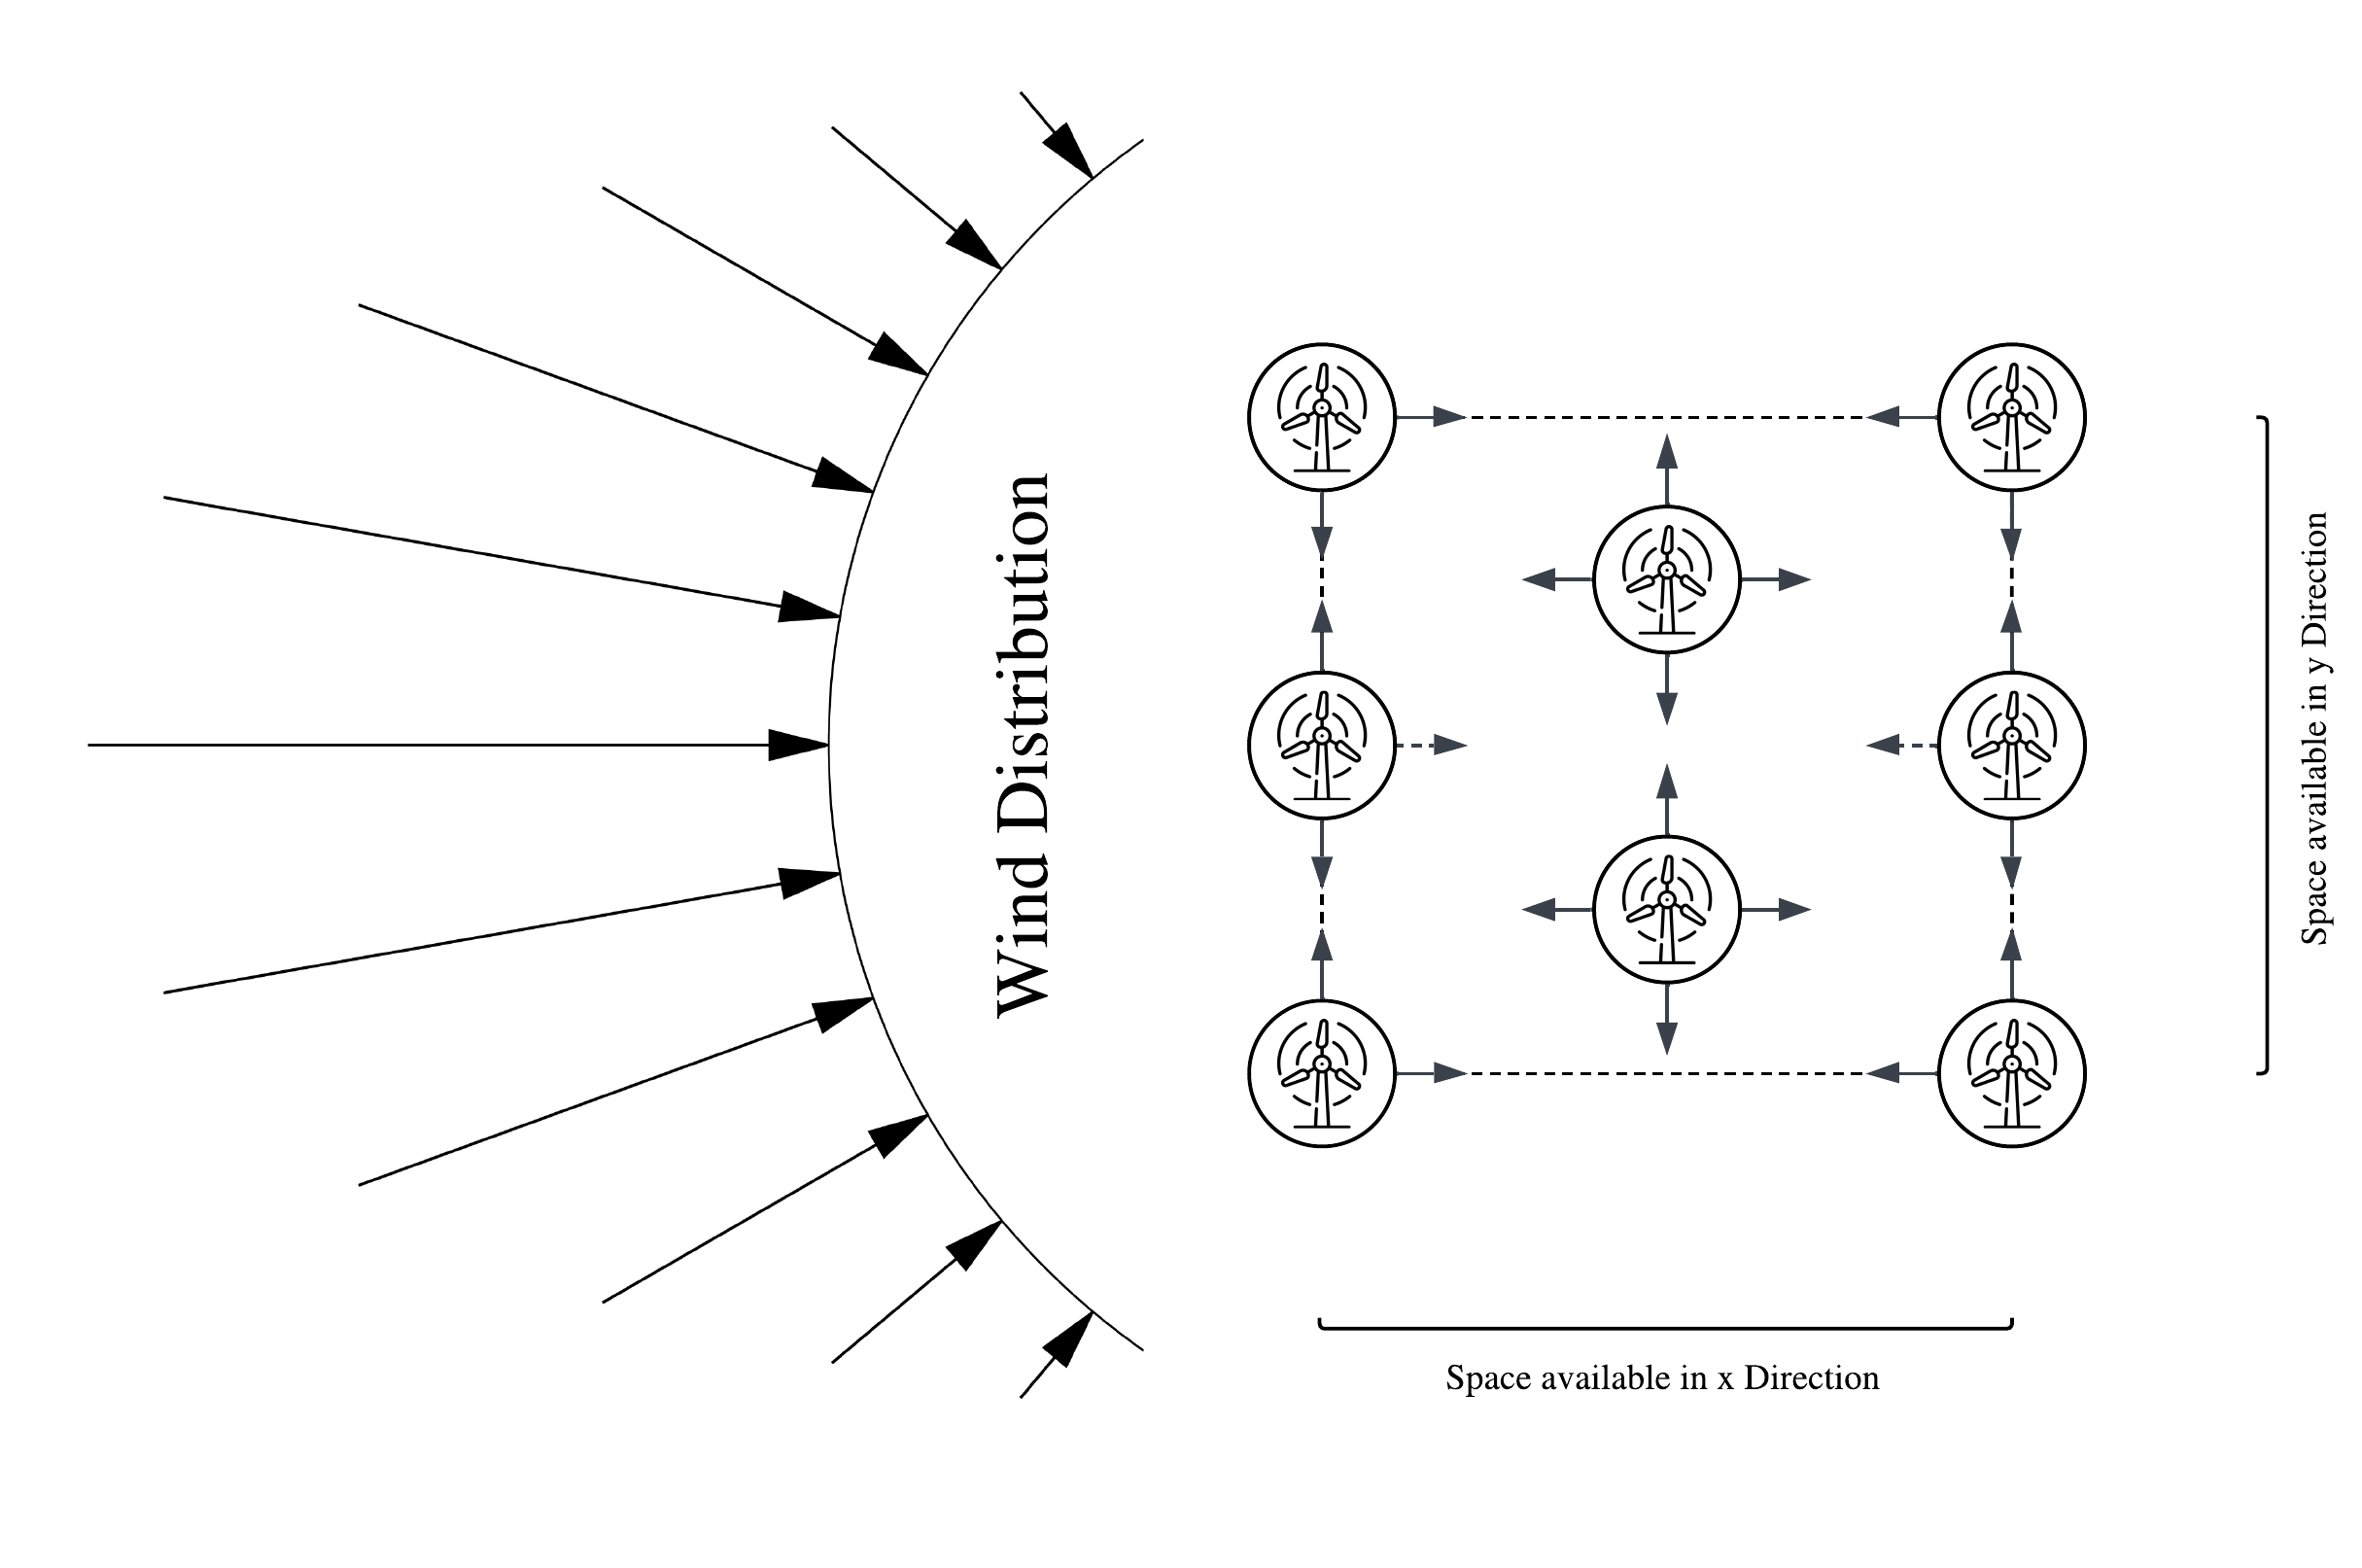
\includegraphics[width=1\textwidth]{../figures/introduction/intro_plot.png} 
	\caption{Optimizing the total power output of a farm reduces to placing wind turbines within a set space for the farm, subject to the wind conditions at the given location}
	\label{fig:intro_plot}
\end{figure}

In mathematical terms, this problem can be expressed as the attempt to maximize the sum of power output across all turbines, e.g., maximizing total farm output, subject to the limitations of the defined space, which is assumed to be rectangular: 

\begin{align}
	\max_{\mathbf{x}, \mathbf{y}} & f_{Power}(x_i, y_i, \text{wind conditions}) \\
	\text{s.t.} \quad 
	&  0 \leq x_i \leq X_{\max} \\
	&  0 \leq y_i \leq Y_{\max} \\
\end{align}

where:
\begin{itemize}
	\item \( (x_i,  y_i) \) are the positions of the turbines
	\item \( f_{Power, \text{NN}}(\cdot)\) is a neural network approximating the farm power output, e.g. the sum of power generated by all individual turbines
	\item \(  X_{\max}, Y_{\max} \) define the maximal extension of the space in which the turbines can be placed
	\item \(\textit{wind conditions}\) are the the random variables that represent the wind conditions at a specific location, like wind direction and wind speed with their respective probability distributions 
\end{itemize}


This thesis is dedicated to a new approach for optimizing the placement of a fixed number of wind turbines in a predefined space, beginning with the two-turbine problem, the problem of optimally placing two turbines relative to each other. To solve this optimization problem, an extension to the Pyomo Python library is used, which allows the embedding of Neural Networks into the optimization problem as a set of constraints \cite{ALCANTARA2023120895}. This extension allows the modelling of the effects of wind turbine placement relative to each other on power production. Introducing this model into the problem then allows for the optimization of overall power production across all wind turbines in the wind park.

To create a model optimally fit to the needs of the optimization problem, the model is trained on data specifically generated with the \href{https://www.nrel.gov/wind/floris.html}{FLORIS} \cite{nrel_floris} wind farm simulation tool  for optimal coverage of the optimizations parameter space. To simplify the problem, the surface below the turbines is assumed to be perfectly flat and an equal wind speed is assumed along the entire height of the turbines. Solving the problem can be seperated into two main Steps:

\begin{enumerate}
	\item \textit{Farm Power Model:} Generation of simulation data covering the parameter space and training a Neural Network model with power generation as output
	\item \textit{Optimization:} Setting up optimization problem, embedding of power model and solving
\end{enumerate}

This thesis is structured according to these two main steps, with a brief review of the state-of-the-art in wind turbine placement optimization and constraint learning beforehand. 

%% Use \subsection commands to start a subsection.

\section{State of the Art}\label{chapter:state_of_the_art}

Since the arrival of large-scale wind turbine farm operations as part of energy infrastructure, optimizing the positioning of the individual wind turbines relative to each other to mitigate wake effects and maximize the total power output is the subject of scientific investigation. As this Thesis is an attempt to apply a novel constraint learning method introduced in \cite{ALCANTARA2023120895} to the optimization of wind farm layouts, the following state-of-the-art is split into two pieces:  The first investigates the current relevant publications of wind farm optimization and the second one presents a brief introduction into recent developments in the field of constraint learning. 

\subsection{Optimization of Wind Farm Layouts}

As discussed in the introduction, one of the main goals in the optimization of wind farm layouts is to reduce the negative impact of wake effects between wind turbines \cite{KIM2024123383}. Historically, rule of thumb approaches were used by setting up the layout as a grid  with the distance between wind turbines, with spacing in the dominant wind direction between 8 and 12 times the turbine rotor diameter and spacing perpendicular to the dominant wind direction 4 to 6 times the turbine rotor diameter \cite{AZLAN2021110047} \cite{hou_review_2019}.

These methods have evolved to with pursuing the goal of maximizing the Annual Energy Production (AEP) of wind farms in the context of stochastic optimization as done in \cite{Sinner_2024} \cite{KIM2024123383}. 

The core of any of the most recent optimizations models is a wake model, which becomes part of the objective function to represent the wake effects on power output. These models can be categorized as \cite{WANG2024118508}: 

\begin{enumerate}
	\item Experimental Methods
	\item Numerical modeling
	\item Analytical/semi-empirical modeling
	\item Data-driven modeling
\end{enumerate}

While experimental methods and numerical models might be the most precise models available for wake modeling, one of the challenges that come with the optimization is that the model has to be able to be introduced into the current state-of-the-art solvers as part of an objective function, leading to the prevalent use of analytical wake models like the Gaussian wake model and the 3D wake model  \cite{WANG2024118508}. With advancements in Machine Learning, the field of data-driven modeling is meanwhile expanding, with successful attempts in introducing Neural Networks and other Machine Learning frameworks into optimizations of wind farm layouts. Generally, either experimental data or data from numerical modeling (more prevalent) is used to train  a chosen model type. The resulting model is then introduced into the optimization problem, as done in \cite{YANG2023119240} \cite{wes-9-869-2024} \cite{TI2020114025} \cite{TI2021618}. 

\subsection{Constraint Learning}

The term Constraint Learning, defined as "finding a set of constraints, a constraint theory, that satisfies a given dataset" in \cite{de2018learning}, is the intersection of machine learning and optimization or more in practical terms, the introduction of machine learning models into optimization problems as constraints. As the in Machine Learnin the models learn from a given data set, the constraints resulting from such a model are equally learned. \cite{de2018learning} 

For this Thesis specifically, we consider the uncertainty aware constraint learning method of decomposing a neural network into a set of mixed-integer linear constraints  \cite{ALCANTARA2023120895} \cite{ALCANTARA2025127876}. Similar approaches of embedding machine learning models into optimization problems have been taken for Decision Trees and Random Forests in \cite{preprintBonfiettiEmbeddDecisionTrees} or for Neural Networks(without integer variables required), as done in \cite{dealba2024reformulationembeddingneuralnetwork}. A survey performed by Fajemisin et al.\cite{FAJEMISIN20241} shows how the field is currently emerging with an increase in publications in recent years and most publications revolving around the Embedding of Neural Networks and Decision Trees/Random Forests.



\section{Farm Power Model}\label{chapter:power_model}

The first central component in optimizing the wind farm layout is to generate a data-driven surrogate Model that can be introduced into the optimization problem and solved by a solver. As detailed in the introduction, the goal is to use the distCL extension \cite{alcantara_ruiz_distcl_2022_git} to the Pyomo Python package, using a small Neural Network as a surrogate model. The following chapter documents the steps taken to generate such a model. 
To train a Neural Network, data is required that covers the parameter space of the optimization to prevent extrapolation by the model. Therefore, the chapter starts by explaining how the open-source wind farm simulation tool \href{https://www.nrel.gov/wind/floris.html}{FLORIS} \cite{nrel_floris} was used to generate a datase. Then, the fundamentals of Neural Network architecture and training are briefly introduced, before the pipeline that yields the final model is presented.


\subsection{Data Source}

The power output of wind turbines and wind farms as a whole is fundamentally connected to the aerodynamic conditions in the airflow every wind turbine experiences, with wind speed as the biggest factor relevant to how much power a wind turbine can generate. The main effect reducing the power generated by a wind turbine is to be positioned in the wake downwind of another turbine. This power reduction is primarily a result of the reduction in windspeed joined with the increased turbulence in the wake airflow (see \ref{fig:wake_photo})  \cite{KIRANOUDIS1997439}. Moving further downstream of a wind turbine, the wake gradually mixes with the outer airflow and thus again increases windspeed until the entire airflow reaches a new homogeneous air speed \cite{MAGNUSSON1999169}. Thus, even if a wind turbine is positioned in the wake of another wind turbine, the greater the distance between the two, the less the second wind turbine is affected. Ideally, wind turbines are not positioned in the wake of other wind turbines at all. 

\begin{figure}[h] 
	\centering
	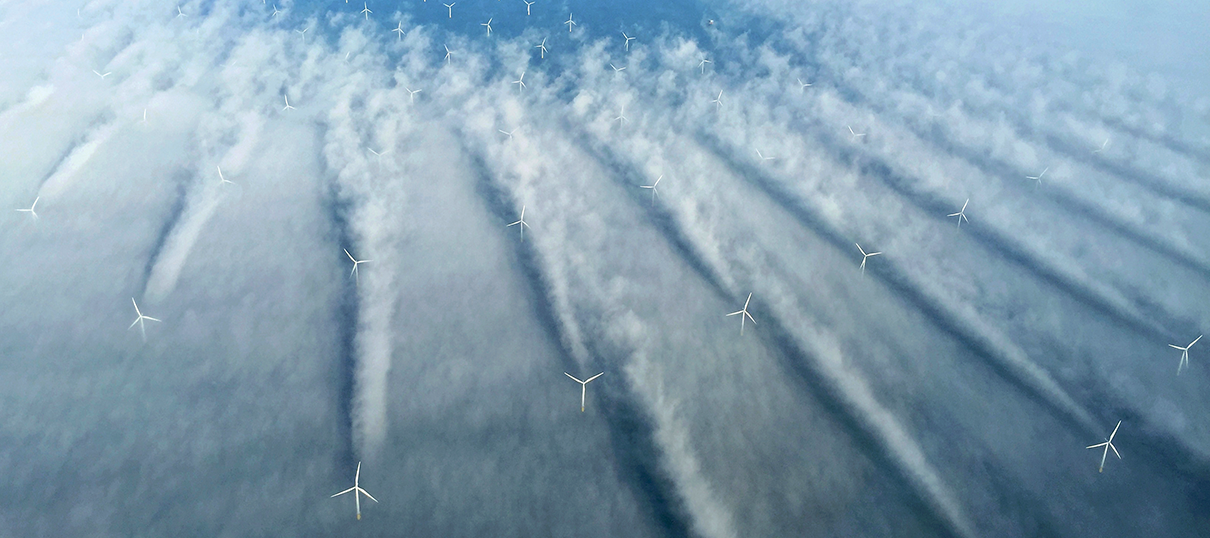
\includegraphics[width=0.8\textwidth]{../figures/introduction/wake_photo.png} 
	\caption{Visible wind turbine wakes due to contrail generation \cite{windpowermonthly_offshore_clusters}}
	\label{fig:wake_photo}
\end{figure}


With the overall goal of creating a model on how the interaction between wind turbines (induced by the wake) is related to the wind turbines relative positioning to each other and the wind conditions as input to an optimization model, a tailor-made dataset from simulation results is the easiest way to ensure that the data fits the use case well. After investigating two Python-based open source wind farm simulation tools FLORIS (\href{https://www.nrel.gov/wind/floris}{FLORIS official website} \cite{nrel_floris_web}) and PyWake (\href{https://topfarm.pages.windenergy.dtu.dk/PyWake/}{PyWake Documentation} \cite{dtu_pywake_2025}), FLORIS was chosen due to its apparent ease of use. FLORIS is a wind farm simulation tool developed by the National Renewable Energy Laboratory (NREL) as one of multiple tools to run simulations of varying complexity. FLORIS is a control-systems-oriented model and therefore contains a lower complexity model yielding fast simulation results. This allows the automatic generation of large quantities of data in a relatively short time. As the data is coming from  simulation results, the data is deterministic even though there is an underlying uncertainty attributed which can be quantified by FLORIS if required. 

For this thesis, FLORIS is given a grid of the following parameters which are dependent on the specific optimization problem:

\begin{itemize}
	\item Position of Wind Turbines
	\item Wind Direction
	\item Wind Speed
	\item Wind turbulence
\end{itemize}

We define the parameter space limits with evenly spaced data points to then generate the corresponding simulation data, with the simulation outputs being the generated power by the individual wind turbines as well as by the farm as a whole (e.g. the sum of individual power outputs). The configuration of all of these parameters, as well as the number of wind turbines, can be modified at will in this setup and the result is a dataset with the rows corresponding to a specific combination of parameters and the resulting power outputs of the turbines. As turbine type, an IEA 10-MW is used for data generation due to its repeated use as a baseline turbine in other scientific works like \cite{Madsen2022} and \cite{Kainz2024IEA} and a more exact technical specification of the turbine can be found in \cite{Bortolotti2019}. The configurations of the specific dataset generated for the individual optimization problem formulations are documented in the corresponding Sections of Chapter \ref{section:optimization}.


\subsection{Introduction to Neural Networks} \label{sec:modelling}

To model the relationship between the attributes of an incoming airflow to a wind turbine and the output generated by the same wind turbine, many surrogate models could be chosen. As the model generated for this thesis is created to be then embedded into the Pyomo extension as explaind in Chapter \ref{chapter:introduction}, the model has to be compatible with said extension. That is why the model chosen is a simple neural network with a limited number of hidden layers and nodes, as large models increase the number of constraints required to decompose the model. 

In the following section, a brief introduction is given to how Neural Networks work and are trained, including some regularization techniques.

\subsubsection{Architecture of a Neural Network}

Fundamentally, Neural Networks represent Graph Networks consisting of function blocks as the nodes, in the case of Neural Networks called "perceptrons" (or Neurons as a more general term) and arcs which correspond to the inputs/outputs of a given perceptron. In simple words, the inputs to the Neurons are summed up and introduced as an argument into a function $f()$, which yields an output $y$ of the given perceptron. These Neurons are organized in layers, which correspond to the row-type structure Neural Networks are usually represented in and each perceptron of one layer is connected to every other perceptron of the following layer. The following layer, in this case, means in the direction of flow, in visualizations usually from left to right. The arcs thus correspond to a single number, and the Neurons to the action of summing up all inputs and then applying the unspecified function $f()$ to generate an output. This process is repeated for all Neurons in the network, with the first layer of the network taking as input the values of the given data features (the input values to the model) and the last layer producing outputs corresponding to the output value(s) of the model. The number of Neurons in this first and last layer corresponds to the task of the Neural Network. If the goal is to identify handwritten numbers 1-9 from 50x50 pixel images, the input layer might have 50x50 Neurons for the value of each pixel, and the output as 9 layers with the output value of each of those last perceptrons representing how much the network "thinks" the given image shows the corresponding numbers 1-9. A schematic of this architecture is given in Figure \ref{fig:neural_network_architecture}.

\begin{figure}[h] 
	\centering
	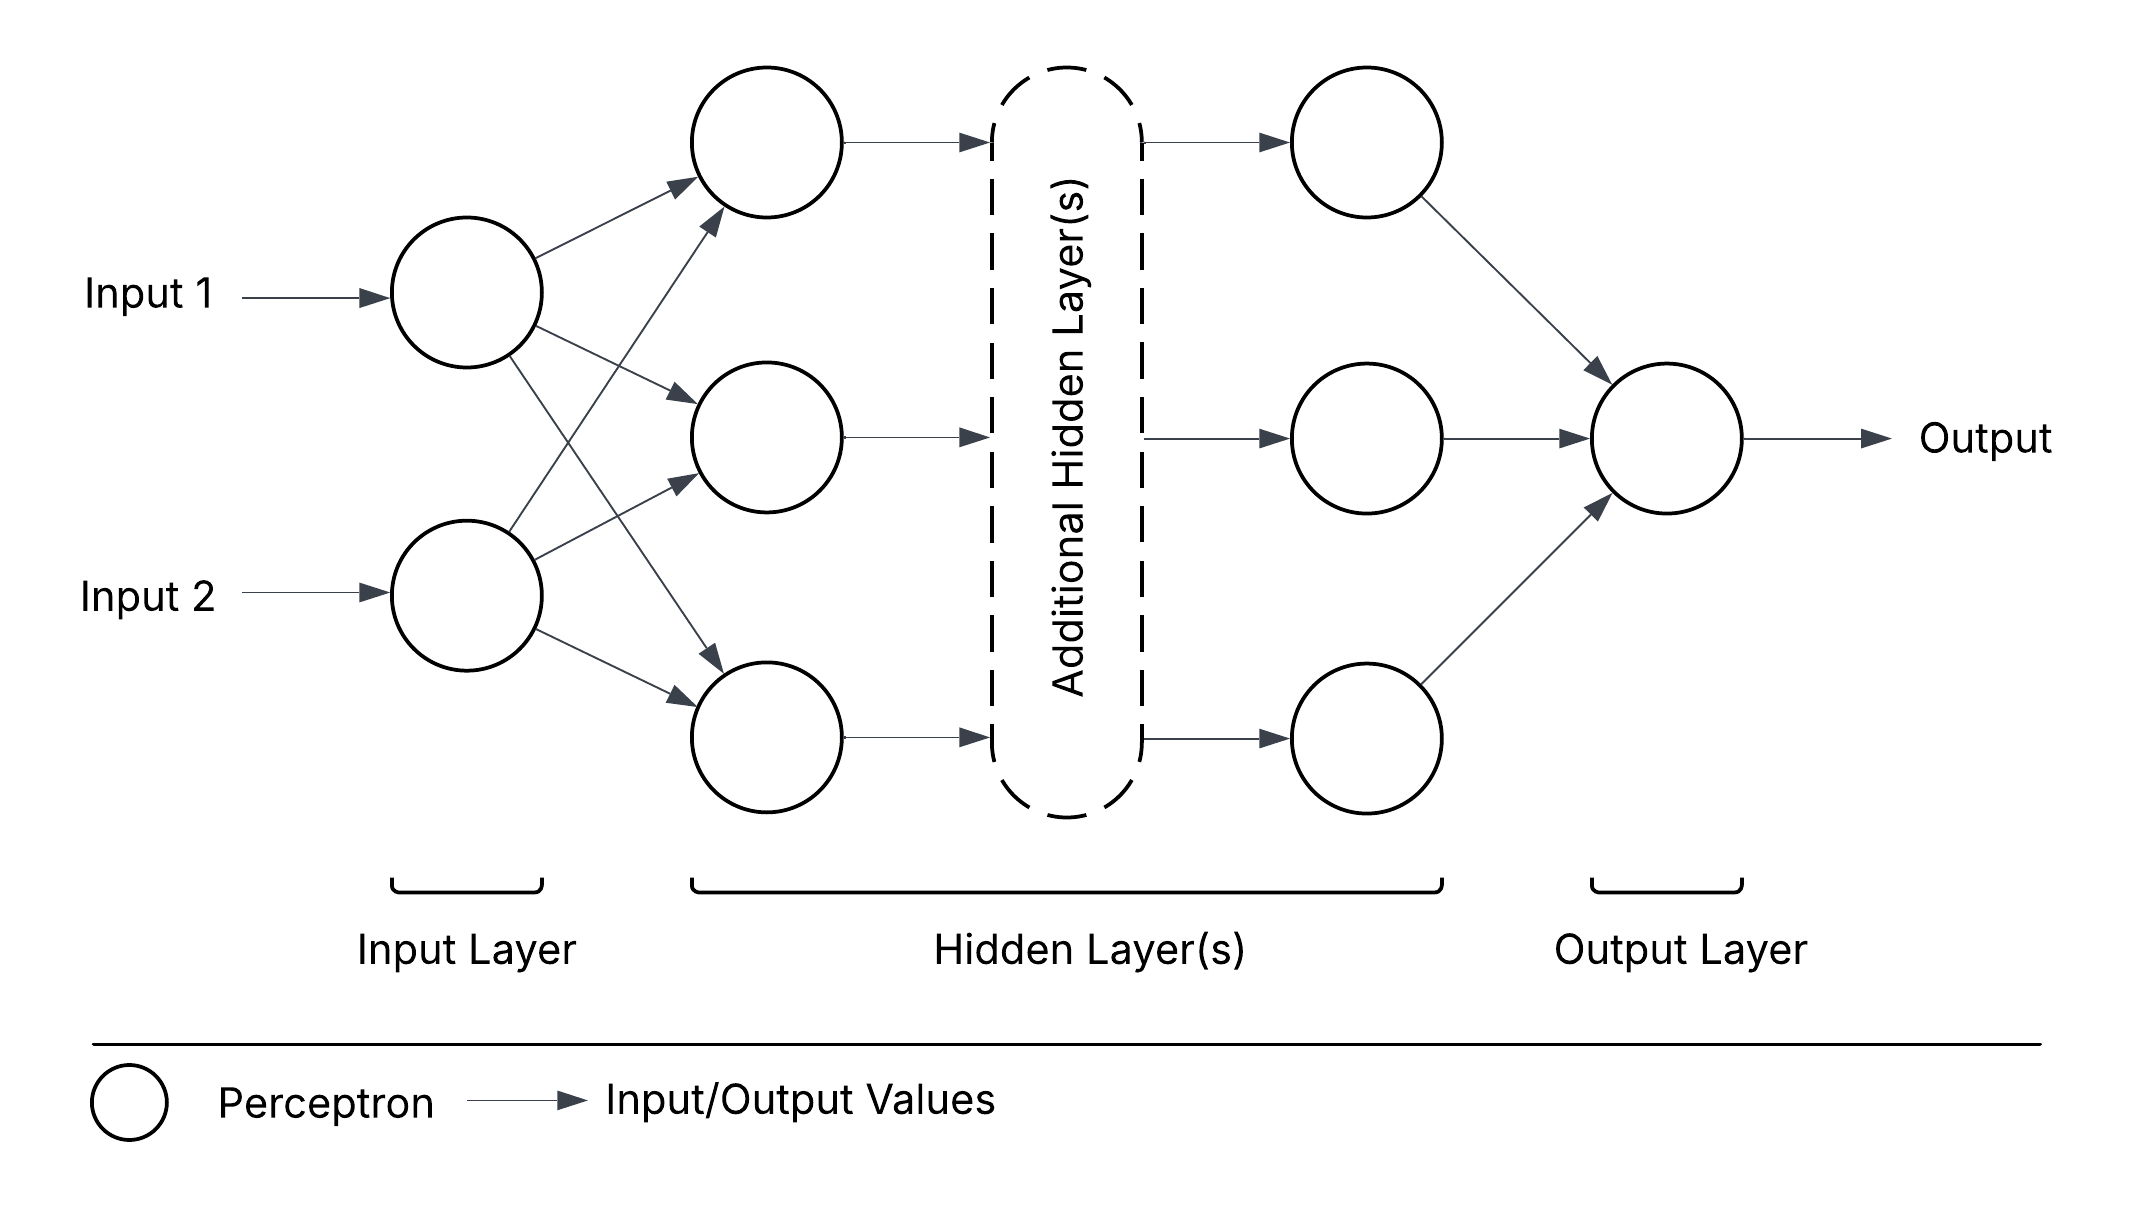
\includegraphics[width=0.9\textwidth]{../figures/modelling/neural_network_concept.png} % file name without extension
	\caption{Schematic of Neural Network Architecture}
	\label{fig:neural_network_architecture}
\end{figure}

As shown in Figure \ref{fig:neuron_calculations} the output of a Neuron is slightly more complicated as described before, as the output $y$ is generated by summing up the inputs $x$ multiplied by a corresponding weight $w$ together with a bias $b$ and introducing this summation as an argument into an activation function $f()$. In this process, the weights $w$ represent a weight to give importance to the individual inputs and the bias $b$ serves to set a minimum output value that will always be reached, regardless of the inputs. 

\begin{figure}[h] 
	\centering
	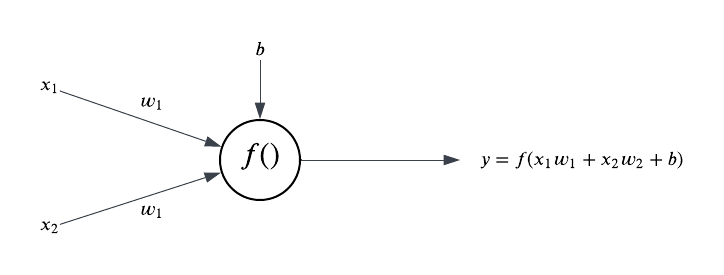
\includegraphics[width=0.8\textwidth]{../figures/modelling/perceptron_concept.png} % file name without extension
	\caption{The output of a neuron is generated by applying the activation function to the sum as the weighted inputs $w_ix_i$ and the bias of the neuron $b$}
	\label{fig:neuron_calculations}
\end{figure}

The function $f()$ is called the activation function, as in its simplest form it represents a step function that decides if a neuron activates or not, e.g., takes the binary values ${0,1}$ for a given threshold. Contrary to the human brain, where neurons are indeed binary, most Neural Networks resort to an activation function whose outputs are not binary but deliver continuous values between $0$ and $1$ to avoid the boundary issues that occur with thresholds. The most common function used in place of a step function is the sigmoid function, which roughly corresponds to a continuous version of the step function, with $\sigma(x) \approx 1$ for $x \to \infty$ and $\sigma(x) \approx 0$ for $x \to -\infty$.


\[
\sigma(x) = \frac{1}{1 + e^{-x}}
\]

This relationship also becomes apparent when plotting both of those functions over each other, as shown in Figure \ref{fig:activation_functions}. 
An alternative to the sigmoid as activation function is the Rectified Linear Unit (ReLu) function, or in simple words, the maximum function, defined as

\[
\text{ReLU}(x) = \max(0, x) = 
\begin{cases}
	0 & \text{if } x < 0, \\
	x & \text{if } x \geq 0.
\end{cases}
\]

The main general applicable benefit of the ReLu function is that it has a constant, non-vanishing gradient for both directions (see Figure \ref{fig:activation_functions}), leading to better gradient propagation, an attribute that is relevant in the context of the backpropagation algorithm briefly discussed in Section \ref{subsubsec:training_nn}. \cite{preprintReLuGlorot}
Beyond this, the ReLu function allows for embedding the Neural Network into a optimization problem, as will be discussed in Section \ref{sec:constraint_learning}.

\begin{figure}[h] 
	\centering
	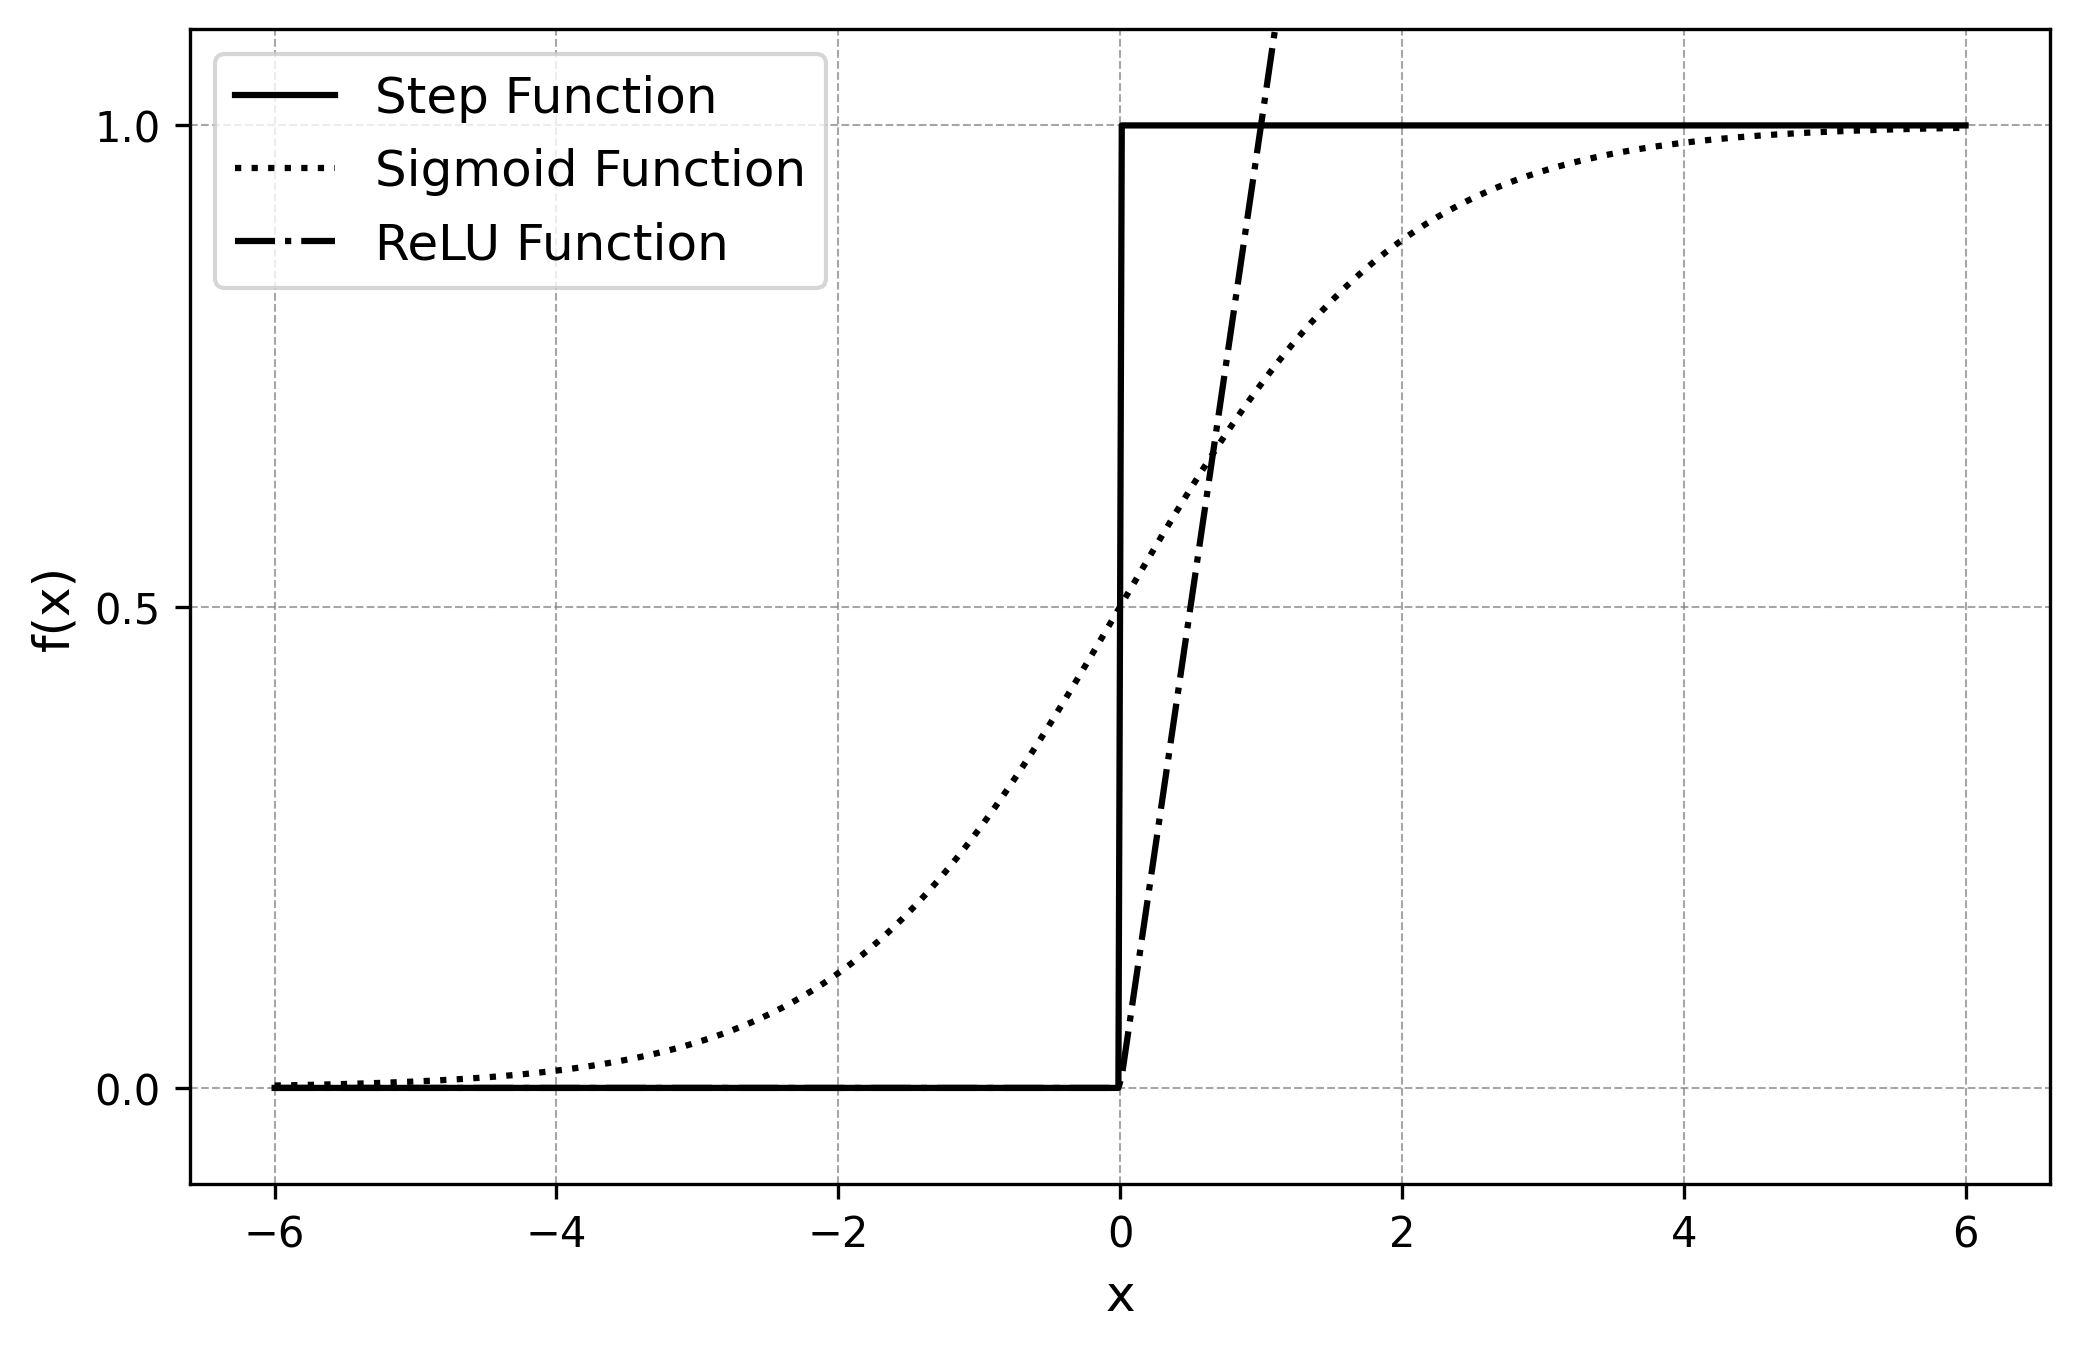
\includegraphics[width=0.9\textwidth]{../figures/modelling/activation_functions.png} % file name without extension
	\caption{The Sigmoid Function being close to the Step Function without being as sensitive to slight changes in $x$ due to its continuity. Alternatively, the Rectified Linear Unit function (ReLu) can be used as activation function. }
	\label{fig:activation_functions}
\end{figure}

\cite{nielsen2015neuralChap1}


\subsubsection{Training a Neural Network} \label{subsubsec:training_nn}

With the general structure set up, and assuming that a layout has been chosen for the neural network (e.g. number of layers and number of their corresponding neurons), the training of the neural network corresponds to adjusting the weights $w$ and the biases $b$ of each neuron in a way, that allows the model to perform the task it is given well. What it means for the model to perform well is defined by a \textit{Loss Function}, which quantifies a relationship between the prediction of the model and the correct output (defined by training data) and gives a Loss as output, which is a sort of difference measure between model prediction and truth. Wether a model is performing well  in a spceific case is heavily dependent on the task (regression, binary classification, multiclass classification, etc.), but regardless of the task, the goal is always to minimize the Loss Function. A well-known Loss Function in regression is the Mean Squared Error (MSE)

\[
\text{MSE} = \frac{1}{n} \sum_{i=1}^{n} (y_i - \hat{y}_i)^2
\]

The training of the Neural Network thus corresponds to adjusting the weights and biases in a way that minimizes the chosen loss function. The algorithm most commonly used for this is called \textit{Backpropagation}.
\cite{nielsen2015neuralChap1}

Before diving into how the algorithms work exactly, it makes sense to first define specifically what parameters have to be optimized, e.g., all weights and biases of the network to be optimized. A common notation of the individual weights is as $w_{jk}^l$ with $l$ being the layer of nodes into which $w_{jk}^l$ are the weights of its inputs (weighing the values from the outputs of the $(l-1)^{th}$ layer) and $j$ as the neuron from the $l^{th}$ layer as well as $k$ the neuron of the  $(l-1)^{th}$. Similarly, the biases are written as $b_j^l$ with $l$ as the layer and $j$ the neuron in that layer as as can be seen for both the weights and bias in an example in Figure \ref{fig:bias_and_weights_notation}.


\begin{figure}[h] 
	\centering
	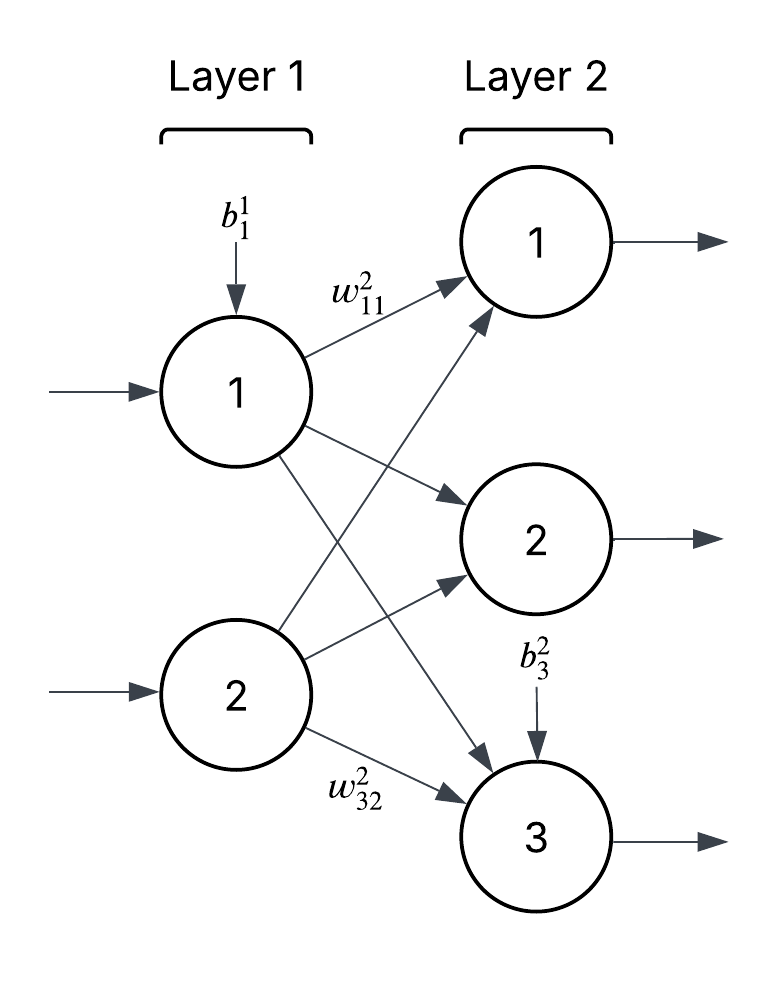
\includegraphics[width=0.4\textwidth]{../figures/modelling/bias_and_weights_notation.png} 
	\caption{Notation of Neural Network weights and biases with weight $w_{jk}^l$ and $l$ being the input layer,  $j$ the neuron from that input layer and $k$ the neuron of the  $(l-1)^{th}$ output layer. Similarly, the bias as $b_j^l$ with $l$ as the layer and $j$ the neuron.}
	\label{fig:bias_and_weights_notation}
\end{figure}

Using this notation, the output of a given neuron $a_j^l$ can be calculated as 

$$
a_j^l = \sigma\left( \sum_k w_{jk}^l a_k^{l-1} + b_j^l \right),
$$

This expression can be further simplified by writing weights and biases in matrix form, using a weight matrix $w^l$ for all weights input into the given layer $l$ and a bias vector $b^l$. By doing so, the output vector $a^l$ of the entire layer $l$ can be calculated as.

$$a^l = \sigma (w^la^{l-1}+b^l)$$

With the notation for weights and biases established, the goal becomes tuning them in such a way as to minimize a chosen Loss function. This is done by using training data with a known true value for the prediction variable and changing weights and Biases in such a way that moves the Neural Network towards outputting the true known value. 
The algorithm to do so corresponds to: 

\begin{enumerate}
	\item Introduce Training Data into the Neural Network
	\item Evaluate the Loss Function for the Training Points (with small random values for weights and biases for the first iteration) and evaluate the gradients of the Loss function for the gradients of the individual weights and biases ($\frac{\Delta Loss}{\Delta w_{jk}^l}$, $\frac{\Delta Loss}{\Delta b_j^l}$) using backpropagation  \footnote{The Gradient can either be evaluated for each training point individually or for batches of training points}
	\item Update the weights and biases according to a learning rate $\rho$ weighted by the specific weight or biases gradient like $w_{jk}^l =w_{jk}^l - \rho \frac{\delta Loss}{\Delta w_{jk}^l}$ and $b_j^l =b_j^l - \rho \frac{\Delta Loss}{\Delta b_j^l}$ 
	\item Repeat process $n$ Epochs, with one Epoch being the algorithm passing through all training points once
\end{enumerate}

This algorithm represents a gradient descent algorithm with learning rate  $\rho$ corresponding to the step length while evaluating the partial derivatives $\frac{\Delta Loss}{\Delta w_{jk}^l}$, $\frac{\Delta Loss}{\Delta b_j^l}$ is the critical step. Here, the backpropagation algorithm gives an efficient method of finding these partial derivatives by evaluating the individual error contributions of each Neuron and how errors accumulate as the inputs move through the Network. A more extensive explanation of how backpropagation works can be found in \cite{nielsen2015neuralChap2}. As is common for gradient descent, finding the global optimum for the weights and biases is not guaranteed and is even improbable if many local minima exist, as they do for the many parameters of a Neural Network. Nonetheless, using gradient descent, it is reasonable to hoped to find a good local minimum as solution \cite{James2023} \cite{nielsen2015neuralChap2}.


\subsubsection{Regularization}

Like most Machine Learning models, Neural Networks run at risk of overfitting. They are especially prone to overfitting due to their many degrees of freedom, represented by the many biases and weights, at times exceeding the number of training samples.

To prevent overfitting, regularization techniques like Cross-Validation can be applied in training, as for any other model. One very specific regularization method for Neural Networks is \textit{Dropout Learning}, which corresponds to randomly removing Neurons from the network (by effectively setting their activation function and thus their output to 0) for each training observation. By other nodes having to "stand in" for the dropped-out nodes, nodes are prevented from developing overspecialization. \cite{James2023}



\subsection{Modelling Pipeline} \label{sec:model_pipe}

With the theoretical foundations laid out, this section is going to treat the actual training process of the Neural Networks to be introduced into the optimization. Part of the challenge of training Neural Networks for this specific purpose is that the objective in optimizing the Neural Network is not only to minimize the cost function, but also to minimize the  number of model parameters, e.g., to minimize the total number of neurons the network consists of. This objective is a result of each neuron corresponding to an additional three linear constraints in the optimization problem, leading the number of constraints to grow as $\Delta n_{constraints} =3 \times \Delta n_{neurons}$. In general, individual models are trained for each optimization problem seen in Chapter \ref{section:optimization} tailored to their individual needs and parameter spaces. This is why this chapter will detail the main components of the modeling process and parameters that will be defined according to the optimization problem later on. The exact configuration of the models will then be defined together with the optimization problem.  

The modelling pipeline contains three main components, with the elements consisting of the data generation, hyperparameter tuning, and the final model training as seen in in Figure \ref{fig:model_flow}. In this case, data generation corresponds to running the required simulations via FLORIS  for the given parameter space, hyperparameter tuning corresponds to the training and evaluation of different model configurations and final model training as the step in which the final model that is to be introduced into the optimization problem is trained (again).


\begin{figure}[h] 
	\centering
	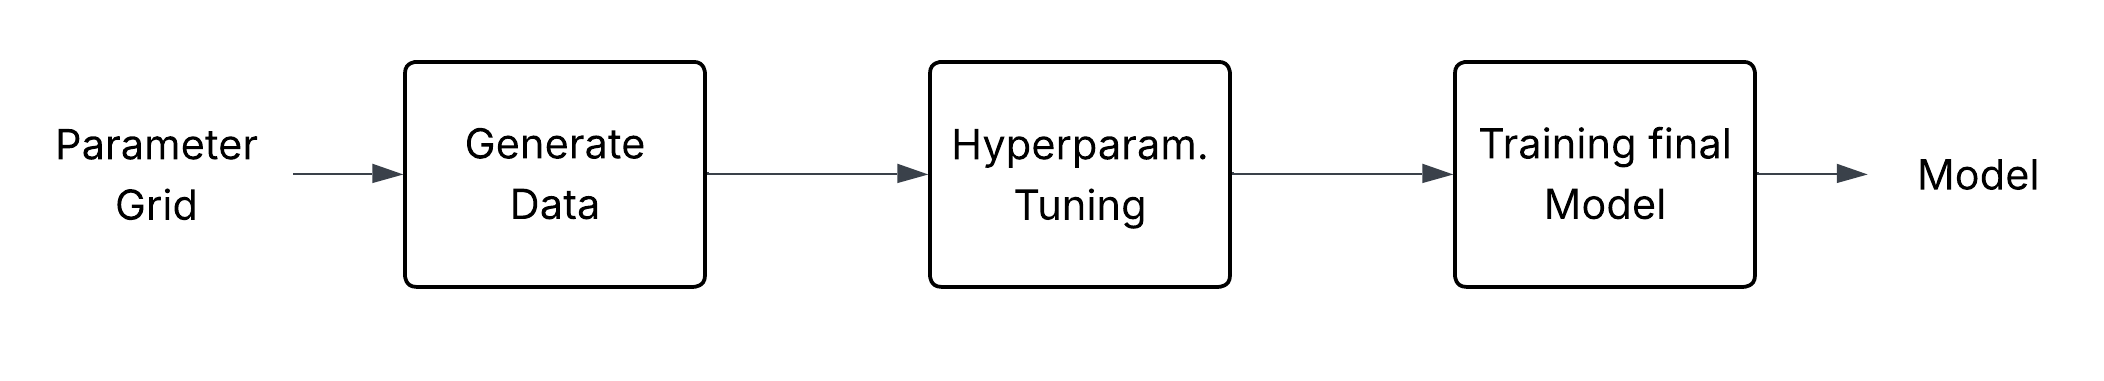
\includegraphics[width=0.9\textwidth]{../figures/modelling/model_flow.png} 
	\caption{Flow of model generation, with parameter grid as input and the final model as output}
	\label{fig:model_flow}
\end{figure}

\subsubsection{Data Generation}

The Data Generation corresponds to the creation of a dataset corresponding to a grid that is set up within the parameter space of the optimization problem. The objective is to generate a dataset that covers the parameter space with sufficient density to train a model that is able to accurately interpolate between the given data points. Each data point corresponds to an individual simulation performed using the tool FLORIS \cite{nrel_floris_web}, allowing for an array of inputs and delivering an array of outputs. As inputs, the following variables can be defined as part of the parameter grid:

\begin{itemize}
	\item x\_range
	\item y\_range
	\item wind\_speeds
	\item wind\_directions
	\item turbulence\_intensities
\end{itemize}

Where x\_range and y\_range correspond to the relative distances of the second wind turbine to the first, wind speed corresponds to wind velocity in m/s,  direction to the incoming wind angle in Degrees (with 0° corresponding to norht, 180° to south) and turbulence intensities as a measure of turbulence for the incoming airflow. Figure \ref{fig:Floris} shows an example of a simulation output. 


\begin{figure}[h] 
	\centering
	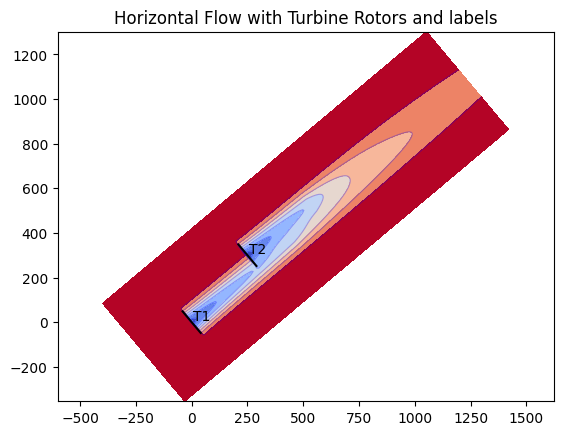
\includegraphics[width=0.7\textwidth]{../figures/modelling/Floris.png} 
	\caption{Example of a Simulation output from the FOLORIS Wind Turbine Simulation Tool \cite{nrel_floris} with colormap corresponding to airflow velocity}
	\label{fig:Floris}
\end{figure}

The method implemented in (\href{https://github.com/schmeti/uc3m_TFM_wind_farm_optimization_codebase/blob/main/Windfarm_power_modelling/generate_data_floris.ipynb}{Data Generation Notebook} \cite{schmetz2025_gendata_git}) takes a range of values together with a specified number of chosen steps for the specific parameter and performs a simulation for all combinations for the given ranges to fill the entire grid. As the number of steps or limits may be different for the different parameters, the grid is not necessarily equally spaced for all parameters, but is constant for each parameter individually, e.g. the distance between values is the same for the entire range.  
Depending on the configuration of the problem, some parameters themselves may be constant. If, for example, a variable like turbulence intensity is not taken into account for a given optimization, a constant value is set, and the data is generated for that constant value. The model trained on this dataset is thus constrained in use to the assumption of that specific constant, a limitation that is important to keep in mind further down the road when the initial dataset generation might not be as conscious anymore. 

The outputs of the simulation are:
\begin{itemize}
	\item Power generated by Turbine 1
	\item Power generated by Turbine 2
	\item Total Power Generation
\end{itemize}

where the total power generation corresponds to the summation of the power generated by the individual turbines. To maximize total farm output, the total power generation will now be used as a target for the model in the following steps.


\subsubsection{Neural Network Configuration}

The next step in the process corresponds to the hyperparameter tuning of the Neural Network. First, an appropriate loss function has to be chosen. The data is then split into a training and an evaluation set, and the model is trained on the training partition using the algorithms detailed in  \ref{subsubsec:training_nn}, using backpropagation/gradient descent as well as dropout learning for regularization for a chosen number of times.  

Once the training process is ended, the model is used to predict for the test partition of the data, and the results are evaluated by scoring the predictions using the Mean Squared Error (RMSE). 

This process is repeated for a grid of the hyperparameters:
\begin{itemize}
	\item Number of Hidden Layers
	\item Number of Nodes in each hidden layer
\end{itemize}

and a plot like shown in Figure	\ref{fig:hyperparm} generated to decide what the best configuration of the Neural Network is. 

\begin{figure}[h] 
	\centering
	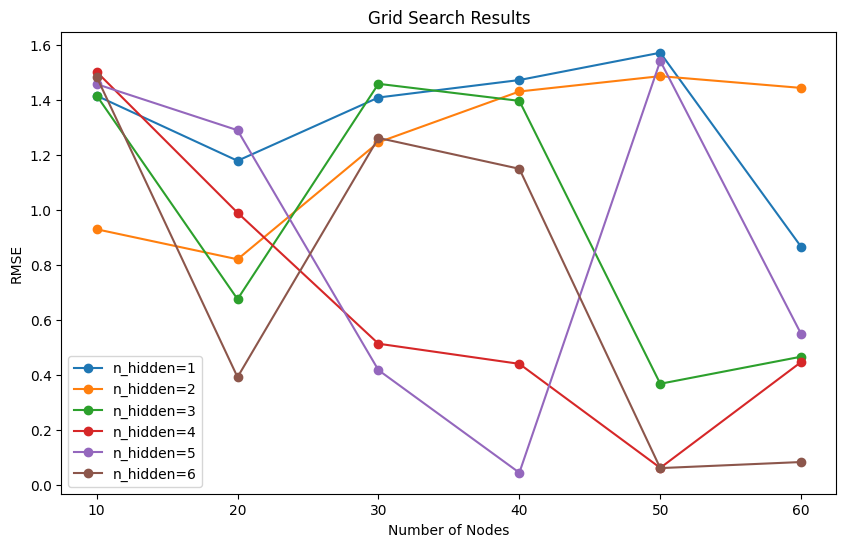
\includegraphics[width=0.8\textwidth]{../figures/modelling/hyperparm.png} 
	\caption{Exemplary Output of Hyperparameter tuning with number of hiden layers $n_{hidden} $ and number of nodes per hidden layer}
	\label{fig:hyperparm}
\end{figure}

The final decision on what the ideal model configuration is, is not only based on the best performance, but via the trade-off between complexity and achieved Loss, to generate a model that is as small as possible.


\subsubsection{Final Model Training}

After having chosen a specific model configuration, a model is then trained using that configuration. This is the model that is eventually introduced into one of the optimization problems detailed in Chapter \ref{section:optimization}.

\subsubsection{Possible Improvements in the Modelling Process}

As one of the two main components of the optimization process, the model generation step shows some potential for improvement in the future. The currently evenly spaced grid of data points could be replaced by a grid that is organically generated according to the gradient of the underlying function by providing a denser grid in areas of large changes in the power function to provide the Neural Network with more data in volatile areas. The result could be an improved accuracy and efficiency, with data points concentrated on areas of interest.   

To reduce the size of the Network, the number of Neurons could be allowed to change from hidden layer to hidden layer to allow for removing expendable Neurons. 

To improve the accuracy of the models, a higher-quality simulation method could be used to generate the dataset. While this might come at a computational cost, the more accurate data might lead to an increase in the  accuracy of power output prediction, which, depending on the application context, might be worthwhile.  

Beyond these two proposals, it is safe to assume that a wide range of methods are available to improve performance and efficiency. These might be worthwhile to pursue once the method developed in this thesis has been shown to provide a valuable new approach to wind turbine positioning optimization.

\section{Optimization}\label{section:optimization}

With the theoretical and pratical foundations of the model of farm/turbine power established, the following section treats the embedding of the trained model(s)  into a deterministic/stochastic optimization problem. The underlying theory of optimization under uncertainty and constraint learning is introduced before the actual optimization problems for the two turbine optimization problem are defined, the required models trained, and the results discussed.


\subsection{Optimization under Uncertainty}

Like in many areas, knowledge about the uncertainty associated with certain variables can change decisions in which these variables underlying uncertainty plays a part. For example, while optimizing anything from next year's crop to tomorrow's energy pricing, the field of Stochastic Programming is occupied with finding methods that allow for introducing these uncertainties into optimization problems.

One way to approach these uncertainties is to split the problem into scenarios. A bakery, for example, has to decide on how many Baguettes to bake for the next day to maximize its profit. Baking too few Baguettes will lead to missing out on potential sales, while baking too many baguettes will mean that the demand is fulfilled, but the money invested in the excess number of baguettes is lost. Assuming the mean number of baguettes bought every day is $1000$, the price to buy a baguette is $1 €$ and the cost to produce a baguette is $0,2 €$ the classical approach to solving such a problem would be by the following formulation \footnote{$x$ of course non-negative}: 


\begin{align*}
	\max_{x} \quad \left( 1.00 \cdot \min(x,1000) - 0.20 \cdot x \right)
\end{align*}


To represent uncertainty, additional scenarios of the demand being $10\%$ lower ($900$ Baguettes) and $10\%$ higher ($1100$ Baguettes) can be added. Assuming that the mean demand has a $50\%$ probability of occurring, the $10\%$ demand increases a $20\%$ probability and the $10\%$ decrease a $30\%$  probability, the problem can be modified to maximize the expected profit across these three scenarios by the formulation

\begin{align*}
	\max_{x} \quad & 0.5 \cdot \left(1.00 \cdot \min(x,1000) - 0.20 \cdot x \right) \\
	&+ 0.3 \cdot \left(1.00 \cdot \min(x,900) - 0.20 \cdot x\right) \\
	&+ 0.2 \cdot \left(1.00 \cdot \min(x,1100) - 0.20 \cdot x\right)
\end{align*}

Assuming only these three scenarios are possible, the result from this optimization problem would be the Expected profit and how many Baguettes are the optimal number of Baguettes to yield the maximum Expected profit across all scenarios. This would be optimal assuming there is no more information about the next day's demand, meaning that by using this approach, the total profit over a long time would be maximal. In case there is more information regarding the next day's demand, the probabilities that give the weights in this optimization might shift, with one scenario potentially reaching probability $100\%$ if there were to be absolute certainty that the next day's demand would be, for example, $1100$ baguettes. As having such exact information is very rare, the best solution will be in most cases to maximize the profit Expectation. 

The obvious connection to conventional statistical analysis is that the demand is a random variable that can take multiple values, in this case, we assumed it to be a discrete random variable $Y$ with support ${900,1000,1100}$ even though in real-world applications the demand of baguettes will move somewhere between $[0,\infty]$. Finding the Expectation for such a discrete random variable can be done as 

\[
\mathbb{E}[X] = \sum_{i} x_i \cdot \mathbb{P}(X = x_i) = \sum_{i} x_i p_i
\]

or for continuous random variables  

\[
\mathbb{E}[X] = \int_{-\infty}^{\infty} x \cdot f_X(x) \, dx
\]

Using these two expressions, optimization problems can thus be formulated to optimize the Expectation of objective functions containing random variables. \cite{BirgeLouveauxStochasticProgramming}


\subsection{Constraint Learning} \label{sec:constraint_learning}

Constraint learning refers to introducing a model that has learned relationships between certain variables from data into an optimization problem. In the case of constraint learning, the model is more specifically introduced into an optimization problem as a set of constraints. As many real-life relationships are dificult to represent by a simple analytical function, introducing machine learning models to optimization problems opens up many new possibilities \cite{FAJEMISIN20241}.

In the case of Neural Networks, one way of introducing a Neural Network as a constraint into an optimization problem is by recognizing that when using the Rectifier Linear Unit (ReLu) Function as activation function with the (linear) sum of neuron bias and weighted inputs $\tilde{v}_i^\ell$ being the function argument


\begin{equation}
	v_i^\ell = \max(0, \tilde{v}_i^\ell) = \max(0,  b_i^\ell + \sum_j w_{ij}^\ell v_j^{\ell - 1})
\end{equation}


the function can be rewritten as the following constraints 

\begin{align}
	v_i^\ell &\geq \tilde{v}_i^\ell \\
	v_i^\ell &\leq \tilde{v}_i^\ell - M^{\text{low}}(1 - j_i) \\
	v_i^\ell &\leq M^{\text{up}} j_i
\end{align}

with $j_i \in \{0,1\}$ a integer variable such that

\begin{align}
	j_i =
	\begin{cases}
		0 & \text{if } \tilde{v}_i^\ell < 0 \\
		1 & \text{if } \tilde{v}_i^\ell > 0
	\end{cases}
\end{align}

This decomposition allows for introducing a Neural Network into an optimization problem by decomposing it into the shown set of mixed-integer linear constraints \cite{ALCANTARA2023120895}.

\subsection{The Two Turbine Problem}

Optimizing the positioning of two wind turbines can be expressed as optimizing the relative position of a second wind turbine $T_2$ to a fixed first turbine $T_1$, defined by the relative distances $\Delta x$ and  $\Delta y$. Both  $\Delta x$ and  $\Delta y$ are constrained by minimum distance $\Delta_{min}$ to  $T_2$ and maximum distances $\Delta x_{max}$/$\Delta y_{max}$ to make the problem bounded. 
This problem can be visualized as shown in Figure \ref{fig:two_turbine_problem}.

\begin{figure}[h] 
	\centering
	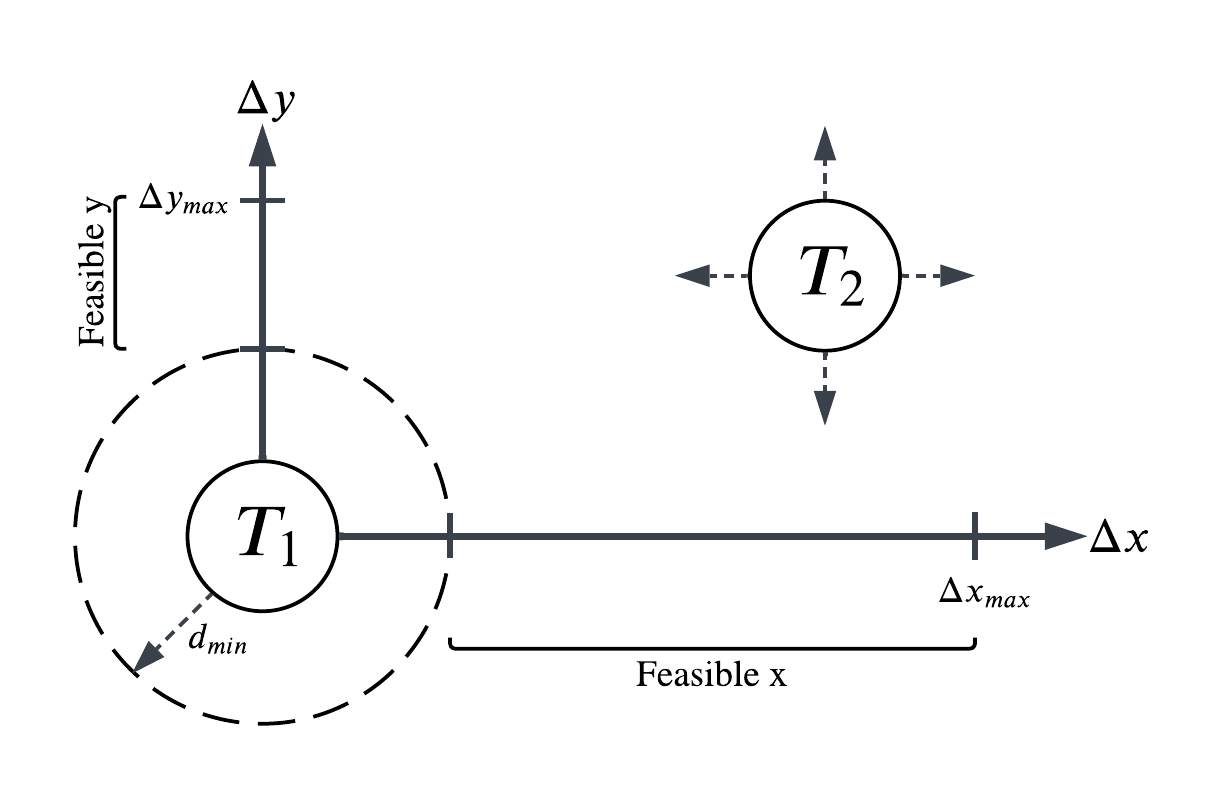
\includegraphics[width=0.6\textwidth]{../figures/optimization/two_turbine_problem_schematic.png} % file name without extension
	\caption{Optimizing the relative position $\Delta x$/$\Delta y$ of a second wind turbine $T_2$ to a fixed first turbine $T_2$, constrained by minimum distance $d_{min}$ to  $T_1$ and maximum distances $\Delta x_{max}$/$\Delta y_{max}$}
	\label{fig:two_turbine_problem}
\end{figure}

The objective function to be optimized is the total power generation, e.g. the sum of power generated by both turbines. This objective is a function of both the position of the wind turbine as well as of the wind conditions like wind direction and wind speed. 

$$
f_{total Power}(x,y,\text{windspeed},\text{wind direction}, \text{(...)})
$$

Different from the geographic coordinates, the wind condition parameters like windspeed are inherently not deterministic and follow distributions like the normal distribution as shown in Figure \ref{fig:wind_dist}.

\begin{figure}[h] 
	\centering
	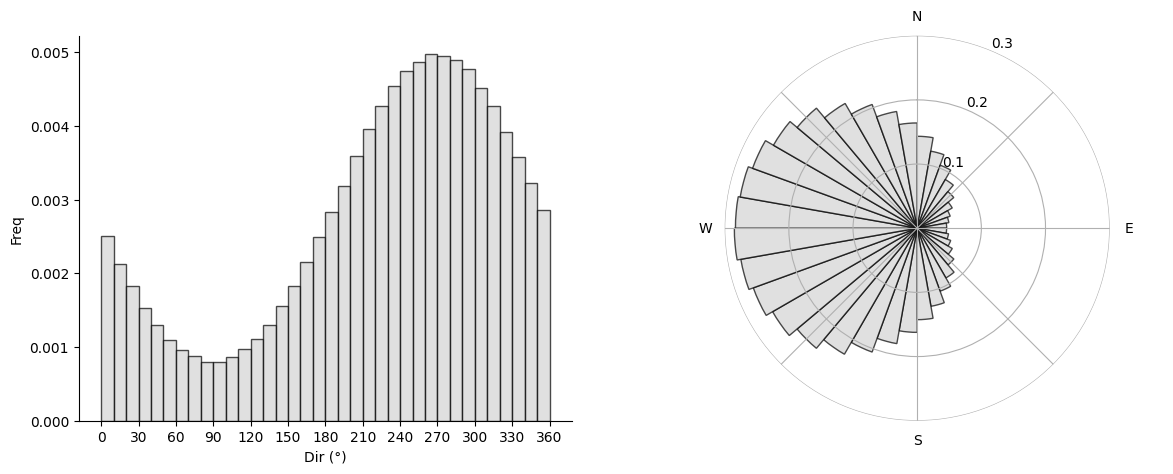
\includegraphics[width=0.9\textwidth]{../figures/optimization/wind_dist.png} % file name without extension
	\caption{Histogram and Polar Plot across radiants for a normally distributed wind direction probability density function with mean West}
	\label{fig:wind_dist}
\end{figure}

The two main challenges of the optimization of the two-turbine problem are thus: 

\begin{enumerate}
	\item Introduce the complex relationship between turbine position, wind conditions, and power output into the optimization problem
	\item Introduce the non-deterministic nature of wind conditions into the optimization problem
\end{enumerate}

The first of these challenges is tackled by applying the Neural Network models discussed in Section \ref{sec:modelling} and introducing them into the optimization problem via constraint learning as described in Section \ref{sec:constraint_learning}. For the second problem, multiple approaches are now explored in the following subsections.


\subsubsection{Deterministic Optimization}

To begin solving the problem, the simplest approach is to assume the wind conditions to be discrete. In application, this might be analogous to using the Expectations of the joint probability distribution of all wind condition parameters, which in pratical terms would be considered the "principal wind direction". Taking these parameters as constant and homogeneous across the entire parameter space, the result is an objective function that is effectively only dependent on the relative positions of the turbine with the previously discussed geometrical constraints.

\begin{align}
	\max_{\mathbf{x}, \mathbf{y}} & f_{Power,\text{NN}}(\Delta x, \Delta y) \\
	\text{s.t.} \quad 
	&  0 \leq \Delta x \leq X_{\max} \\
	&  0 \leq \Delta y \leq Y_{\max} \\
	& \sqrt{(\Delta x)^2 + (\Delta y)^2} \geq d_{\min}
\end{align}

where:
\begin{itemize}
	\item \( (\Delta x, \Delta y) \) are the relative distances of the two turbines
	\item \( f_{Power, \text{NN}}(\Delta x, \Delta y)\) is a neural network (deterministic) approximating the total farm power output
	\item \(  X_{\max}, Y_{\max} \) define the maximal distance the two turbines can be placed apart
	\item \( d_{\min} \) is the minimum distance between the two turbines
\end{itemize}



The Notebook belonging to this formulation can be found in \href{https://github.com/schmeti/uc3m_TFM_wind_farm_optimization_codebase/blob/main/Windfarm_power_modelling/0_two_turbine_problem_constrLearn_determin.ipynb}{Deterministic Fomulation Notebook} \cite{schmetz2025twoturbine_determ}

\paragraph{Modelling}

To begin with, the simulations to generate the dataset used to train the corresponding model for the deterministic case have to be generated. For the deterministic optimization, the position of the second turbine is variable in the given bounds and with an even steplength  as shown in Table \ref{tab:val_determ_data}. All remaining airflow characteristics remain constant (deterministic).

\begin{table}[ht]
	\centering
	\caption{Value Ranges for Deterministic Two Turbine Problem Data Set}
	\begin{tabular}{|l|c|c|c|}
		\hline
		\textbf{Variable} & \textbf{Const/Variable} & \textbf{Value} & Step Length\\
		\hline
		$\Delta x_{\text{turb2}}$ & Variable & [0, 5000] m & 50 m\\
		$\Delta y_{\text{turb2}}$ & Variable & [0, 500] m & 50 m \\
		wind\_speed & Constant & 8 m/s & -\\
		wind\_direction & Constant & 270°&- \\
		turbulence\_intensity & Constant & 0.06 & - \\
		\hline
	\end{tabular}
	
	\label{tab:val_determ_data}
\end{table}

In line with the parameter space defined in Table \ref{tab:val_determ_data}, simulations are performed as described in Section \ref{sec:model_pipe}. The resulting dataset is then introduced into the Neural Network optimization method, yielding Figure \ref{fig:determ_nn_opti}. When considering the results, it is apparent that models with a number of layers greater or equal than two and greater or equal than 8 nodes per hidden layer are nearly identical in performance. \textit{The chosen model configuration is therefore a $\text{NN}(5\,{-}\,8^{\times2}\,{-}\,1)$}, yielding good performance while reducing model size as much as possible, to be implemented in the optimization problem. 

\begin{figure}[h] 
	\centering
	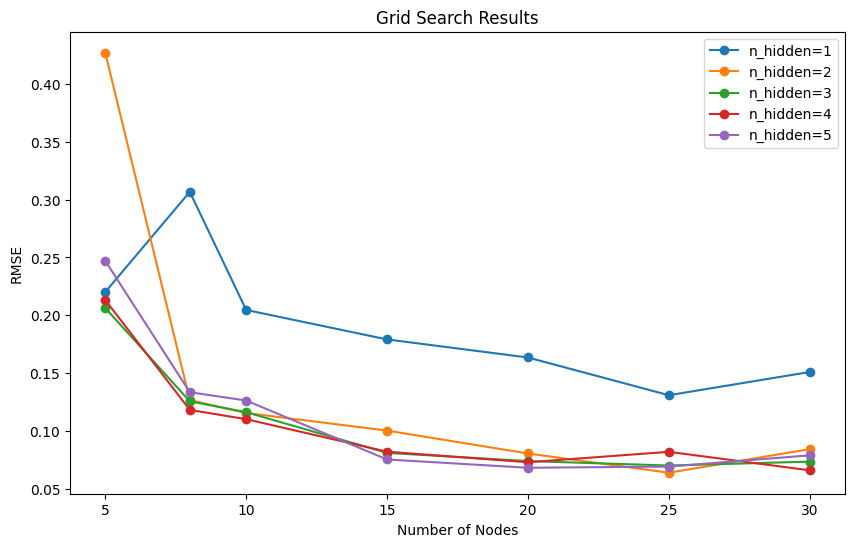
\includegraphics[width=0.7\textwidth]{../figures/optimization/determ_nn_opti.png} 
	\caption{Grid search for Neural Network parameters for the deterministic model, showing how models with $n_{hidden} \geq 2$ and $n_{nodes} \geq 8$ yield near identical performance}
	\label{fig:determ_nn_opti}
\end{figure}

To validate the chosen model and gain a deeper understanding of its predictive power, we proceed to visualize the total power output across the variable parameter space. Figure \ref{fig:determ_model_colormap} shows a colormap generated from linealy interpolating between the datapoints for the simulation data (Subplot 1), a finer grid of predictions of the model (Subplot 2) and a colormap of the percentage deviation between model prediction and true simulation values (calculated at points and then again linearly interpolated). The color in the first two subplots represents the \textit{total power generated of both wind turbines}, with the second turbine placed at the given x/y location We find that the model appears to overall represents the behaviour well, with only systematic deviation occuring at locations very close to the first wind turbine at the origin. As the simulation allows for placing wind turbines at the exact same location and with corresponding results unrealistic, simulations in this area are not necessarily correct in results either. For the optimization, the minimum distance constraint removes this area from the feasible region, meaning that the comparatively large deviations there do not affect the optimization. 

\begin{figure}[h] 
	\centering
	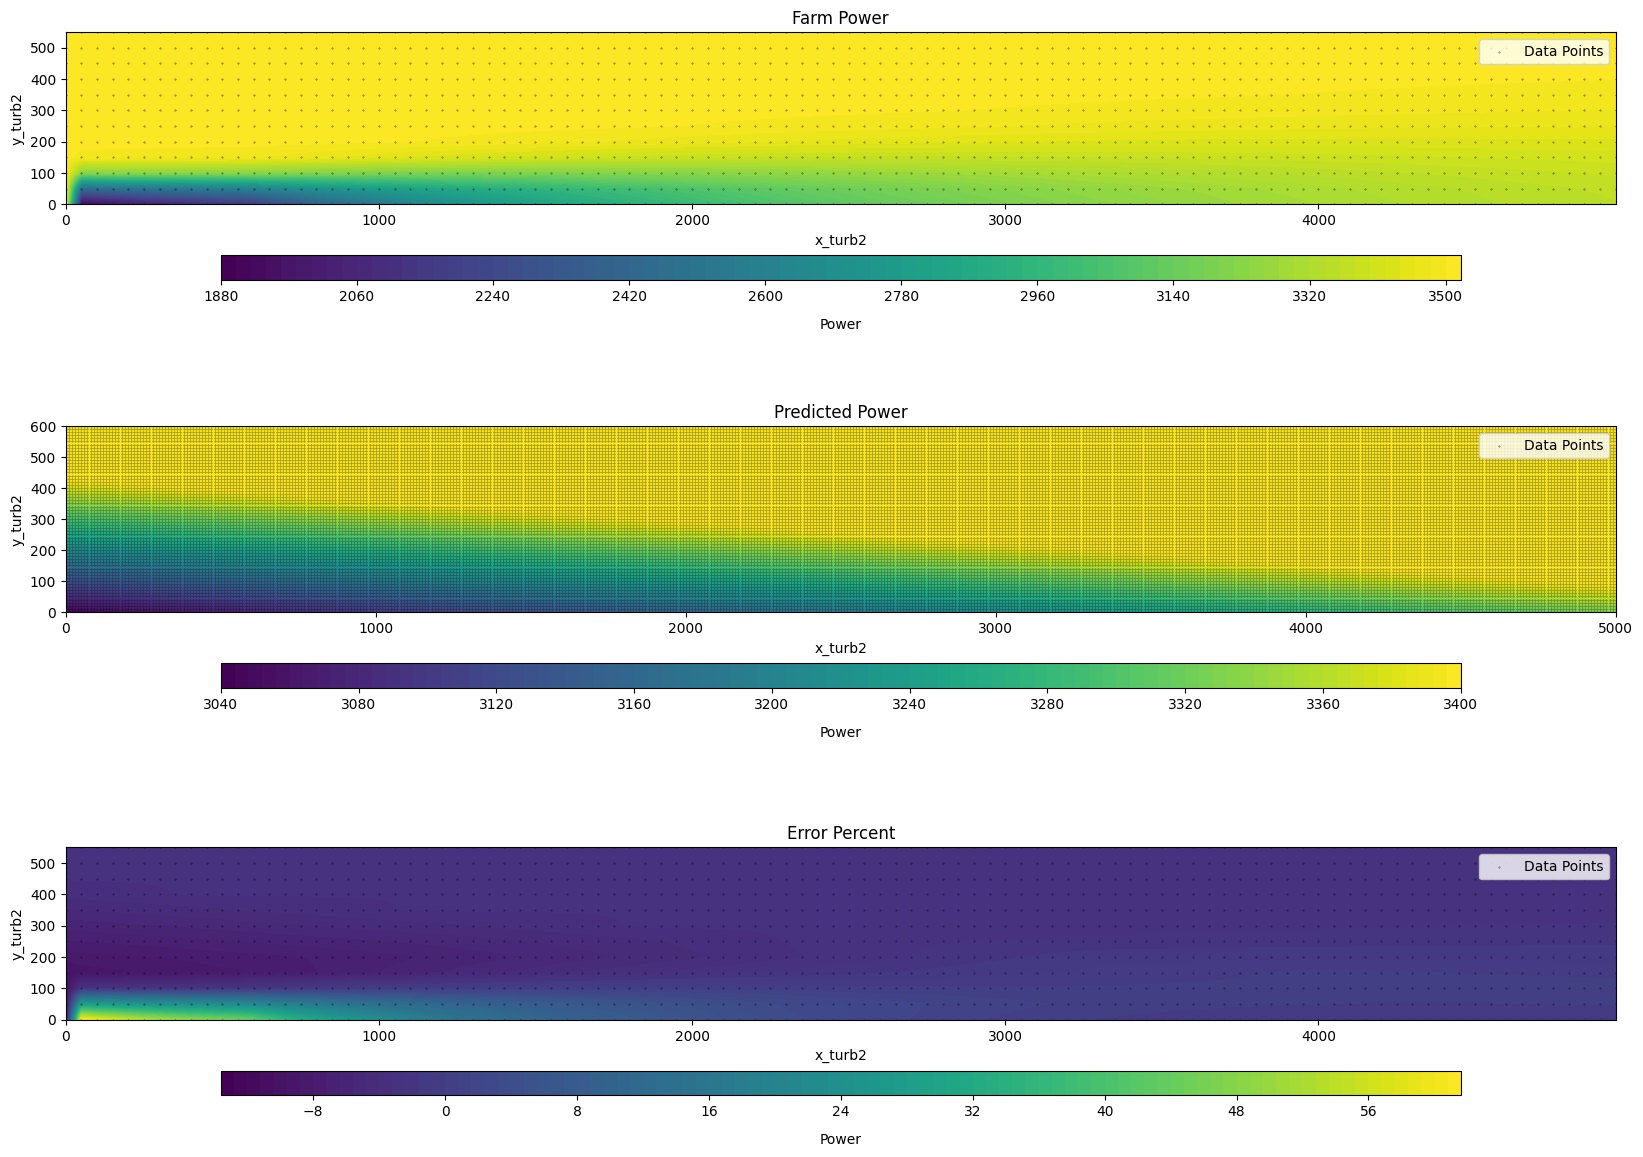
\includegraphics[width=1\textwidth]{../figures/optimization/determ_model_colormap.png} 
	\caption{Colormap showing the Farm Power distribution for the second turbine being placed at any given x/y based on linear interpolation for real data, predicted data and the resulting percentage deviation, indicating overall good fit with only area of major deviation extremly close to turbine 1, an area excluded from the feasible region of the optimization problem }
	\label{fig:determ_model_colormap}
\end{figure}

The model thus appears to be suitable to represent the interactions between the two turbines and we proceed to the optimization.

\paragraph{Optimization}


With the model trained and validated, we proceed to implementing the defined optimization problem in Pyomo  and embed the trained model using the approach described in Section \ref{sec:constraint_learning}.

When solving this problem as defined using Gurobi, a major challenge becomes apparent as the result shows that there is an large number of equally optimal solutions (e.g. degeneracy of the problem, see  \cite{vanderbei2020chapter3} for an exact definition of degeneracy) everywhere outside the wake of turbine 1, as can be seen  in the visualization of the optimization result found in \ref{fig:opti_determ270}.


\begin{figure}[h] 
	\centering
	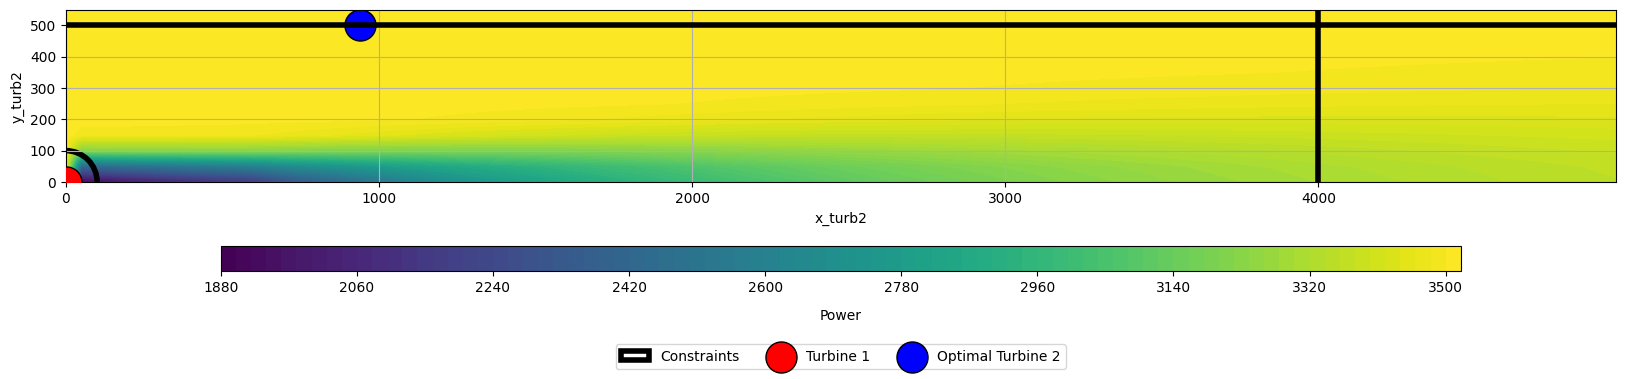
\includegraphics[width=1\textwidth]{../figures/optimization/opti_determ270.png} 
	\caption{Deterministic optimization of the relative position of two wind turbines relative to each other with wind direction 270° and constant windspeed}
	\label{fig:opti_determ270}
\end{figure}

The existence of a large number of optimal values thus has to be taken into account moving forward.

\subsubsection{Stochastic Optimization} \label{sec:stoch_opti_1}

As the deterministic optimization does not account for the distribution of wind condition parameters and has found that the deterministic approach leaves a range of infinite global optima outside of the wake of turbine 1, the next step is to proceed with the introduction of uncertainty of the wind condition parameters into the problem. To do so, the objective function is modified to represent the expected power generated by the farm, if a turbine were to be placed at a given location. The Neural Network thus now has to be able to predict the power output for a given turbine 2 location, taking into account the wind condition parameters like direction and speed at a given location. The problem is formulated as follows: 

\begin{align}
	\max_{\mathbf{x}, \mathbf{y}} &  \sum_{i=1}^{n} f_{Power,\text{NN}}(\Delta x, \Delta y, \text{wind condition})\cdot p_{n,\text{wind condtion combination}} \\
	\text{s.t.} \quad 
	&  \Delta x \leq X_{\max} \\
	&  \Delta y \leq Y_{\max} \\
	& \sqrt{(\Delta x)^2 + (\Delta y)^2} \geq d_{\min}
\end{align}

Where:
\begin{itemize}
	\item \( (\Delta x, \Delta y) \) are the relative distances of the two turbines,
	\item \( f_{Power, \text{NN}}(\Delta x, \Delta y)\) is a deterministic neural network  approximating the total power output for turbine positions and wind conditions
	\item \(  X_{\max}, Y_{\max} \) define the maximal distance the two turbines can be placed apart
	\item \( d_{\min} \) is the minimum distance between the two turbines
	\item \(p_{n, \text{wind condtion combination}}\) is the probability corresponding to each of the scenarios
	\item \( n \) is the index of the discretized possible combinations of wind conditions 
\end{itemize}

The following section will first treat the univariate case of only wind direction being random, while wind speed and turbolence intensity remain constants. 


The Notebook belonging to this formulation can be found in \href{https://github.com/schmeti/uc3m_TFM_wind_farm_optimization_codebase/blob/main/Windfarm_power_modelling/0_two_turbine_problem_constrLearn_probweighted.ipynb}{Stochastic optimization with farm power NN Fomulation Notebook} \cite{schmetz2025twoturbine_stoch1}

\paragraph{Modelling}

Like for the deterministic case, we begin by finding a fitting Neural Network model that can be embedded into the optimization problem. To do so, we again define the parameter space, this time with wind direction being variable and set up in a grid with step length of 10°. The full parameter grid is defined in Table \ref{tab:val_prob_data}

\begin{table}[ht]
	\centering
	\caption{Value Ranges for Probabilistic Two Turbine Problem Data Set}
	\begin{tabular}{|l|c|c|c|}
		\hline
		\textbf{Variable} & \textbf{Const/Variable} & \textbf{Value} & \textbf{$Steplength$}\\
		\hline
		$\Delta x_{\text{turb2}}$ & Variable & [0, 5000] m & 50 m\\
		$\Delta y_{\text{turb2}}$ & Variable & [0, 500] m  & 50 m\\
		wind\_speed & Constant & 8 m/s & -\\
		wind\_direction & Variable & [180°, 270°]& 10° \\
		turbulence\_intensity & Constant & 0.06 & - \\
		\hline
	\end{tabular}
	\label{tab:val_prob_data}
\end{table}

We then proceed to hyperparameter tuning of the model. Due to the added complexity, the model size has to be increased significantly to yield similarly good results compared to the deterministic case. As apparent in Figure \ref{fig:determ_nn_opti}, the performance appears to flatline for models with or more than 2 layers and with or more than 50 nodes, yielding similar performance. To minimize the number of nodes, we thus proceed with the initial model configuration $\text{NN}(5\,{-}\,50^{\times2}\,{-}\,1)$ for the following optimization.


\begin{figure}[h] 
	\centering
	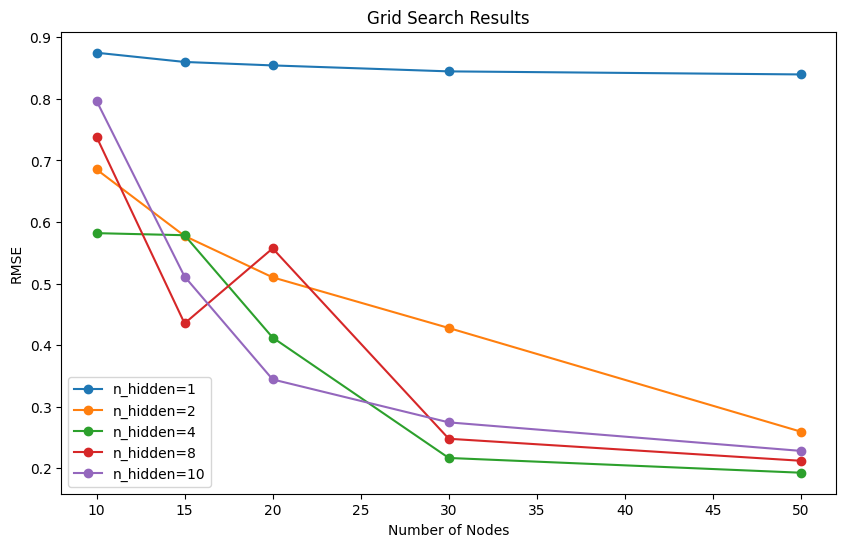
\includegraphics[width=0.62\textwidth]{../figures/optimization/prob_nn_opti.png} 
	\caption{Grid Search results for a Neural Network configuration to predict for data with variable wind direction, showing similar performance for models of layers greater or equal than two, starting at 50 or more nodes}
	\label{fig:determ_nn_opti}
\end{figure}


With a model chosen, we again investigate its performance and find that even with the significantly more complex model, the results are not as good as for the model only trained for the deterministic case. While visually the shape of the wake generally appears to fit, the deviation in percent shows greater deviation, especially at greater distances away from Turbine 1 for the case of wind direction 260°, as shown in Figure \ref{fig:prob_model_colormap}. The model appears to also show some artifacts, with the most notable being the highest values in parallel to the wake right at the borders of the wake flow itself.

\begin{figure}[h] 
	\centering
	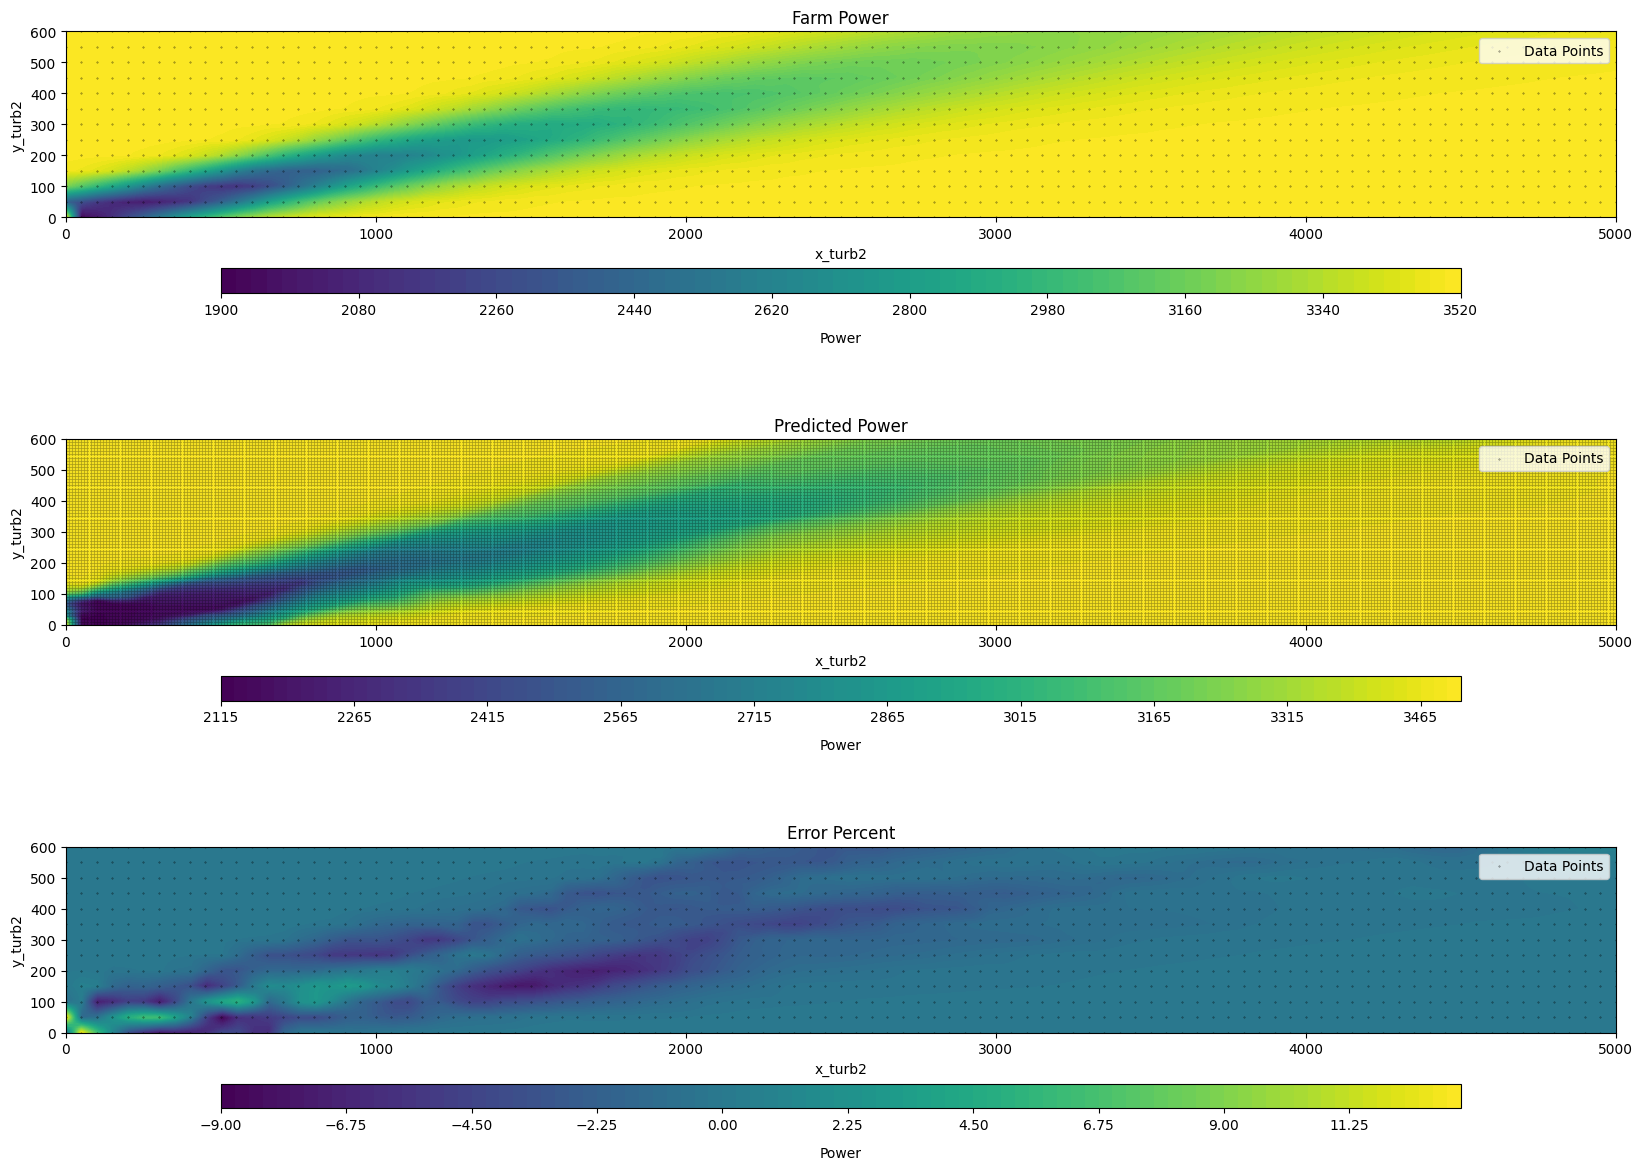
\includegraphics[width=1\textwidth]{../figures/optimization/prob_model_colormap.png} 
	\caption{A heatmap of total generated farm power for a wind direction of 260° with datapoints and linear interpolation in between. Plot 1 shows the raw data, plot 2 the predictions of the $\text{NN}(5\,{-}\,50^{\times2}\,{-}\,1)$, plot 3 the percentage difference between training points and predictions}
	\label{fig:prob_model_colormap}
\end{figure}

Having observed the deviation described above, another layer is added to the model in an attempt to prevent the previous behaviour. The resulting configuration $\text{NN}(5\,{-}\,50^{\times3}\,{-}\,1)$ improved the previous models weaknesses in that respect as can be seen in Figure \ref{fig:prob_model_colormap_2}, which is why \textit{the final model choosen for the optimization is  $\text{NN}(5\,{-}\,50^{\times3}\,{-}\,1)$}

\begin{figure}[h] 
	\centering
	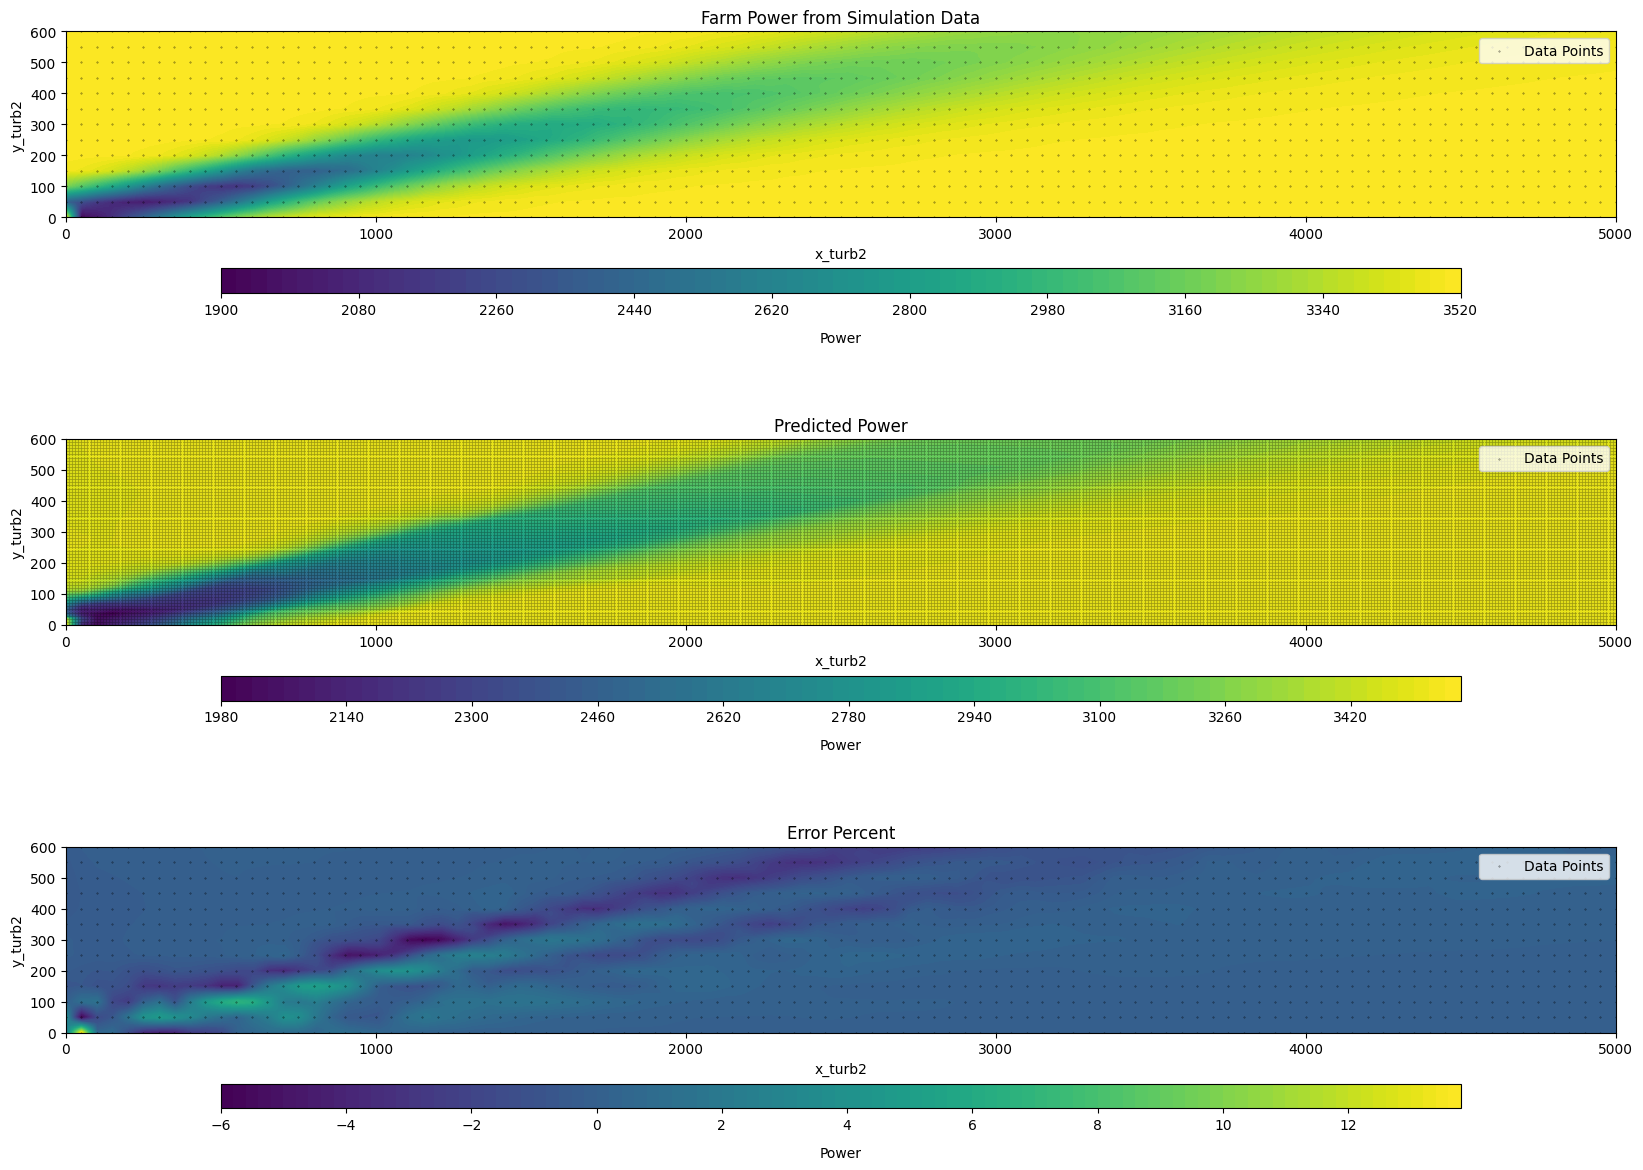
\includegraphics[width=1\textwidth]{../figures/optimization/prob_model_colormap_2.png} 
	\caption{A heatmap of total generated farm power for a wind direction of 260° with datapoints and linear interpolation in between. Plot 1 shows the raw data, plot 2 the predictions of the $\text{NN}(5\,{-}\,50^{\times3}\,{-}\,1)$, plot 3 the percentage difference between training points and predictions, overall showing improved }
	\label{fig:prob_model_colormap_2}
\end{figure}

Since the parameter space has now become three-dimensional, conditioning on a single wind direction does not cover the full performance of the model. Figure \ref{fig:rmse_dist_3layers50nodes} shows the development of RMSE across different wind directions, indicating that the border regions and wind directions with an increased total wake length (e.g. wind directions closer to 270° wind direction) experience higher RMSE, providing more space for errors to accumulate. 

\begin{figure}[h!] 
	\centering
	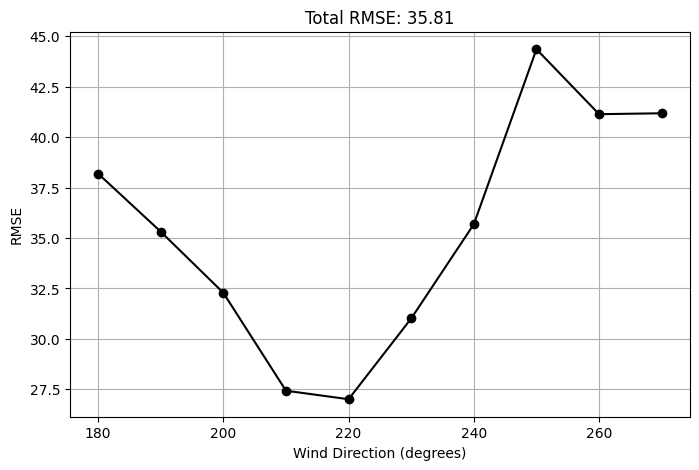
\includegraphics[width=0.55\textwidth]{../figures/optimization/rmse_dist_3layers50nodes.png}
	\caption{RMSE of  $\text{NN}(5\,{-}\,25^{\times10}\,{-}\,1)$ across the parameter space of wind direction }
	\label{fig:rmse_dist_3layers50nodes}
\end{figure}

While increasing the size of the Neural Network might further reduce the deviations across wind directions and for the individual wind directions, it is restricted by the solvability of the optimization problem. While there is no exact threshold, the solving time of the mixed integer problem that results from the embedding of the Neural Network increases roughly exponentially by adding Neurons to the Network and therefore adding binary variables to the problem. The shown model is deemed sufficient because of that trade-off.

For optimization purposes, the individual power per wind direction becomes less relevant, as the power outputs are weighted by their probability of occurring. 
To do so, first the probability distribution of the wind directions has to be defined, like the Normal distribution with mean 270° and standard deviation of 10° shown in Figure \ref{fig:wind_dist_opti}. To calculate the expectation for the discretized parameter space using the trained model, this distribution itself has to be discretized in line with the initial parameter space defintion, which in this case is done in 10° steps. 


\begin{figure}[h] 
	\centering
	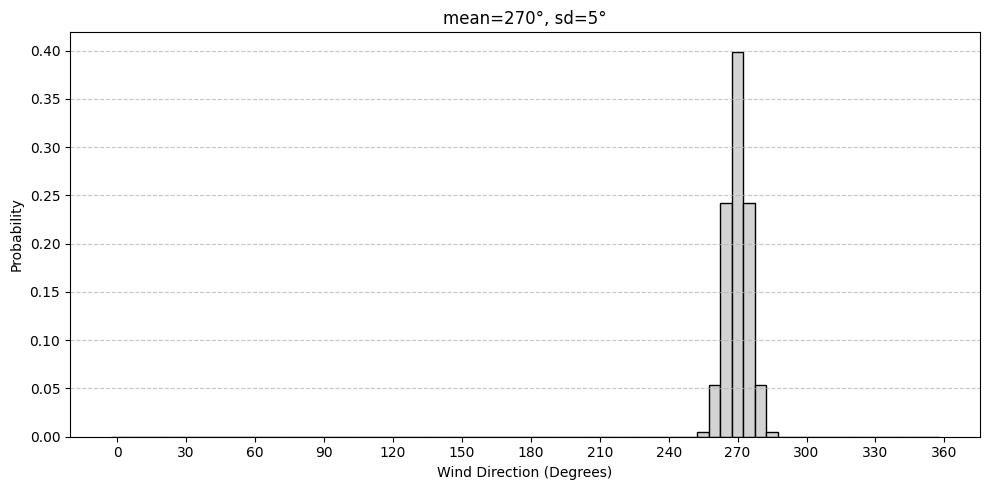
\includegraphics[width=1\textwidth]{../figures/optimization/wind_dist_opti.png} 
	\caption{Discrete Wind Direction Probability Distribution with mean 270° and standard deviation 5°, discretized in intervals of 10° }
	\label{fig:wind_dist_opti}
\end{figure}


Using this distribution, the expected power for the ranges of x and y coordinates can thus now be calculated by aggregating the powers for the different wind directions as a sum weighted by probability to yield the expected farm power generated at the specific coordinate. By evaluating the expected farm power both for the training data as well as for predictions for the training data, we can again compare the results and deviations as done in Figure \ref{fig:prob_expectation}. The directions with a probability greater than are shown as lines and their impact on the distribution of expected farm power visibel.

\begin{figure}[h] 
	\centering
	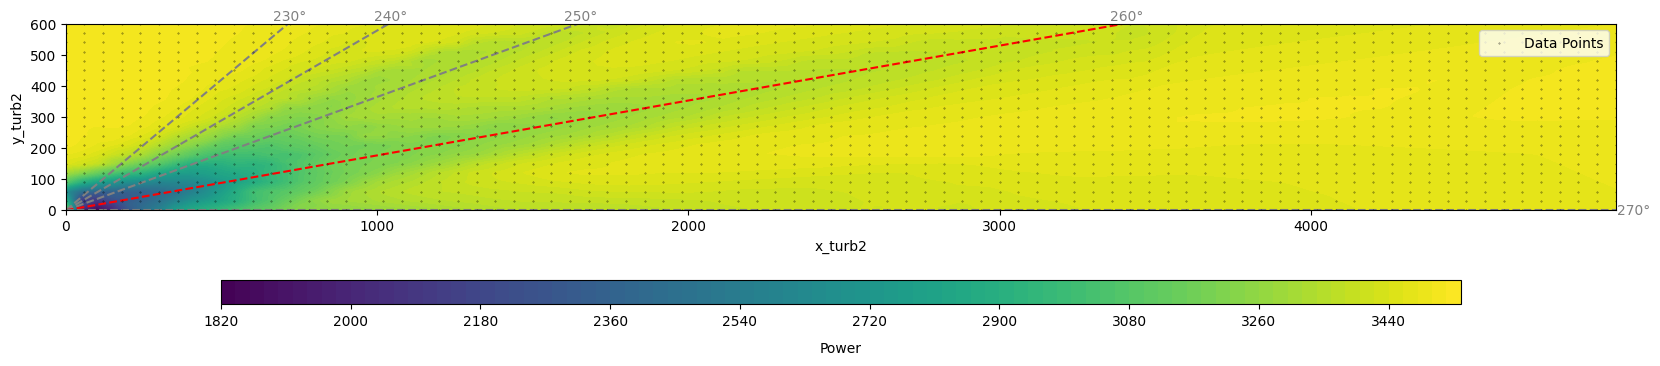
\includegraphics[width=1\textwidth]{../figures/optimization/prob_expectation.png} 
	\caption{Distribution of Expectation of Farm power from a discretized Normal distribution with mean 260° and standard deviation 10° with steplength 10°}
	\label{fig:prob_expectation}
\end{figure}

In the same way the distribution of farm power was previously dependent on the deterministic wind direction, it is now dependent on the wind direction distribution, e.g. its mean and variance, assuming a Normal distribution. Changing the mean of the distribution corresponds to changing the direction of the principal wind direction and thus the direction of the highest expected wake losses from turbine 1. Meanwhile, increasing the variance corresponds to spreading the expected wake losses due to turbine 1 across a wider range of wind directions and therefore increasing the area affected by expected wake losses, while reducing the absolute reduction in expected power within the area affected by the wake. This relationship can be seen in the expected power distribution for a normal with mean 220° and standard deviation 20° shown in Figure \ref{fig:wind_dist_opti2}.


\begin{figure}[h!] 
	\centering
	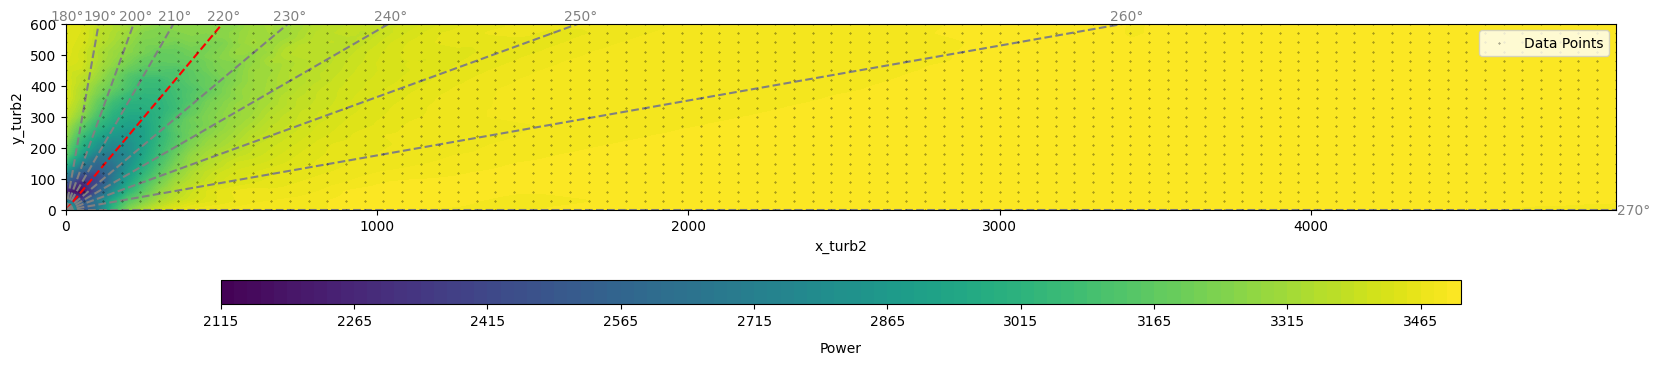
\includegraphics[width=1\textwidth]{../figures/optimization/prob_expectation2.png} 
	\caption{Distribution of Expectation of Farm power from a discretized Normal distribution with mean 220° and standard deviation 20° with steplength 10°}
	\label{fig:wind_dist_opti2}
\end{figure}


The normal distribution is used in this thesis as a placeholder for proof-of-concept purposes. In a practical application, the real wind distribution would have to be evaluated at the specific location of the wind farm. 

\paragraph{Optimization}

With the model set up, solving the stochastic optimization problem for a maximum expected farm power output can be attempted. In the case of optimization, the problem is limited to three scenarios due to the computational constraints due to the size of the problem. A normal distribution with a mean of 270° and  a standard deviation of 5° was therefore used as the wind direction distribution, yielding three scenarios (260°,270°,280°).

The Neural Network and the wind direction distribution are introduced into pyomo to find a global maximum. As previously, a range of optima exists, with Poyomo choosing among this area, as seen in Figure \ref{fig:prob_data_lininter}. More specifically in this case, the area close to the wake had been shown to predict higher values than in the simulations by the model (see Figure \ref{fig:prob_model_colormap_2}), showing the optimization to find the global maximum within the provided Neural Network. 

\begin{figure}[h] 
	\centering
	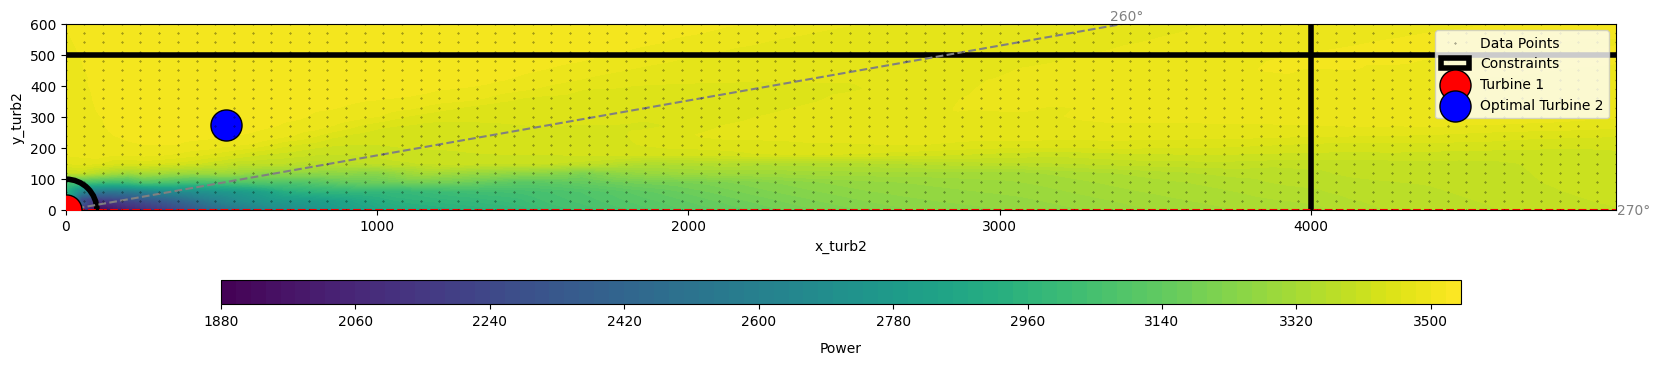
\includegraphics[width=1\textwidth]{../figures/optimization/prob_data_lininter.png} 
	\caption{}
	\label{fig:prob_data_lininter}
\end{figure}

Like before, it is possible to visually find that there is a large range of more or less equally optimal points, with the few scenarios not covering the space appropriately. This leads to seemingly optimal areas in between the scenario wind directions, where in reality, significant wake losses can be expected. In addition to that, some small deviations of the model due to its complexity affect the optimization outcome significantly, with the current model predicting a maximum farm power production for turbine 2 placement close to the wake of turbine 1. Both of those aspects are weaknesses in the current configuration of the stochastic optimization.

\paragraph{Stochastic Optimization: Quantile Discretization of Wind Direction Distribution } \label{subsubsection: discretization}

The first problem observed in this formulation as the gaps between the scenario wind directions as shown in Figure \ref{fig:prob_data_lininter}, can be partially solved by discretizing not with a constant step length but based on the quantiles of the distribution. The discretization can be instead performed not by a constant length of the discretization steps, but by a constant probability within a chosen number of quantiles. For each quantile individually, the mean is then calculated and the resulting expected values for the quantile are taken as discretization steps. This approach, when used for the same Normal distribution with mean 270° and standard deviation 5°, fixing the scenario/quantile count to 7, yields the discretization shown in Figure \ref{fig:wind_dist_opti_quantiles}. 

\begin{figure}[h] 
	\centering
	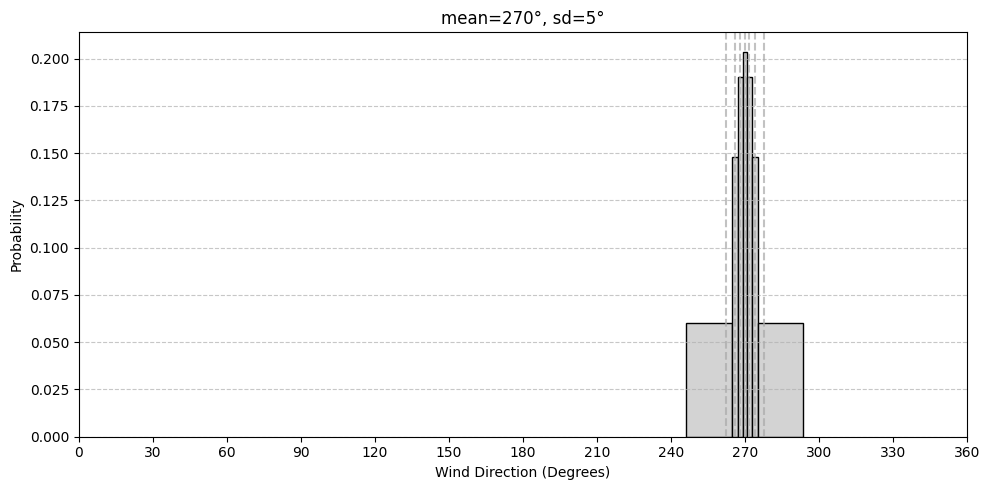
\includegraphics[width=0.8\textwidth]{../figures/optimization/wind_dist_opti_quantiles.png} 
	\caption{Quantile based discretization of Normal mean 270°,  standard deviation 5°, disrcetized into 7 scenarios with equal probability for scenario and the scenario angle corresponding to the expected value for the quantile }
	\label{fig:wind_dist_opti_quantiles}
\end{figure} 

Using this distribution, the expected power distribution changes for the corresponding scenarios/quantiles, with the space left between scenarios proportional to the probability density. When considering the previous approach to stochastic optimization, the number of scenarios that can be introduced into the problem has now become the main limitation. The following subsection provides an alternative set up that allows for a greater number of scenarios.

\subsubsection{Stochastic Optimization: Direct Expectation Neural Network}

While the expectation maximization has shown to be the most accurate depiction of the problem on theoretical level, the previous method used for the resulting stochastic optimzation has shown to be severly limited by computational power, as a large Neural Network is required to model the farm power output both across x and y ranges of the second turbine, as well as across the wind condition variables. 
To overcome these constraints, a alternative formulation is set up, where the Neural Network is designed to output the expected farm power at any x/y point, given a certain wind condition distribution. 



\begin{align}
	\max_{\mathbf{x}, \mathbf{y}} &  \mathbb{E}[f_{Power}(\Delta x, \Delta y) \mid \text{wind condition distribution}]_\text{NN} \\
	\text{s.t.} \quad 
	&  0  \leq \Delta x \leq X_{\max} \\
	&  0  \leq \Delta y \leq Y_{\max} \\
	& \sqrt{(\Delta x)^2 + (\Delta y)^2} \geq d_{\min}
\end{align}

Where:
\begin{itemize}
	\item \( (\Delta x, \Delta y) \) are the relative distances of the two turbines,
	\item \( \mathbb{E}[f_{Power}(\Delta x, \Delta y) \mid \text{wind condition distribution}]_\text{NN}\) a Neural Network that predicts the Expected Farm Power at al \( (\Delta x, \Delta y) \) positions in the parameter space, given a specific wind speed distribution 
	\item \(  X_{\max}, Y_{\max} \) define the maximal distance the two turbines can be placed apart
	\item \( d_{\min} \) is the minimum distance between the two turbines
\end{itemize}

In practice, the new Neural Network configuration is achieved by training the Network directly on the Expected Farm Ppower Values, with the only remaining variables as the relative x/y position of the second wind turbine. To do so, the simulation values across the wind condition variables for a single location are used to calculate the expectation for that location as a probability weighted sum, with probabilities resulting from the distribution of the wind condition variables (wind direction, etc). To combine this approach with quantile discretization from Section \ref{subsubsection: discretization}, the resulting quantile scenario discretization is used to define the parameter space for the initial data set generating simulations. That way, a match between the scenario values and data set discretizations can be assured to allow for seemless calculation of the expectations. 

The central benefit of this formulation is that the dimensionality of the Neural Network is significantly reduced, with only  \(\Delta x, \Delta y\) remaining free after calculating the expectations. The drawback ist that the model is thus condition on a spcific wind condition distribution and can not be used in a more flexible way.


The Notebook belonging to this formulation can be found in \href{https://github.com/schmeti/uc3m_TFM_wind_farm_optimization_codebase/blob/main/Windfarm_power_modelling/0_two_turbine_problem_constrLearn_probweightedt_expNN.ipynb}{Stochastic optimization with farm power Expectation NN Fomulation Notebook} \cite{schmetz2025twoturbine_stoch2}

\paragraph{Modelling}

To generate the model with the farm power expectation as output, more steps are required as initially described in Chapter \ref{sec:model_pipe}. As detailed in the introduction, for the configuration used in this chapter, the Wind Condition distribution, which in this case will only be the distribution of wind directions, has to be defined. For this wind distribution, a discretization is generated the quantile based method described in Section \ref{subsubsection: discretization}. From this discretization, together with chosen limits for \(\Delta x, \Delta y\), the parameter grid/space is defined and corresponding simulation performed to generate the data set. The probabilities from the wind condition distribution are then joined to the dataset and used to calculate the Expected Farm power for each \(\Delta x, \Delta y\) combination in the parameter grid. This yields a significantly smaller data set with \(\Delta x, \Delta y\) and Expected Farm power as features. This dataset is then used to train a model in the same way done previously, choosing a appropriat configuration of the model which then is used for embedding in the optimization problem. The described steps are shown in Figure \ref{fig:stoch2_model_flow}.


\begin{figure}[h] 
	\centering
	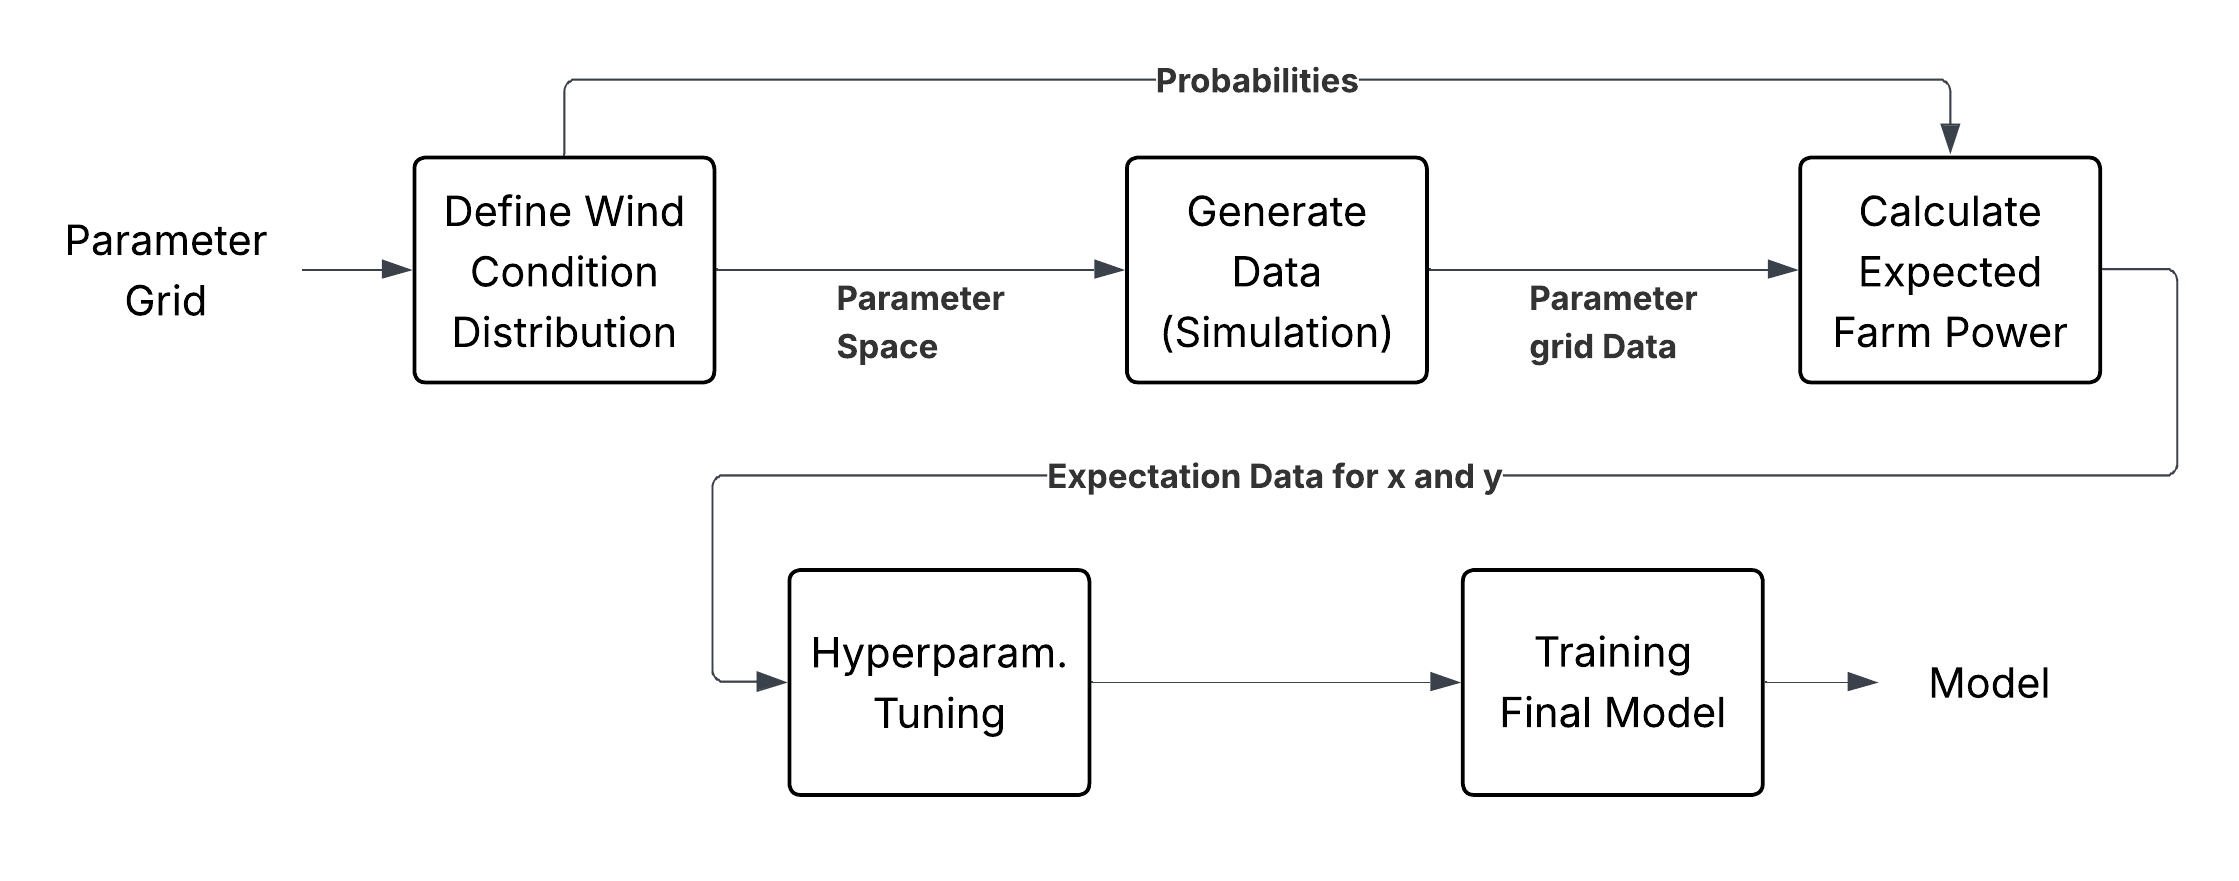
\includegraphics[width=1\textwidth]{../figures/optimization/stoch2/stoch2_model_flow.png} 
	\caption{Flowchart displaying the steps used to set up a Neural Network model to model Expected Farm Power across \(\Delta x\) and  \(\Delta y\)}
	\label{fig:stoch2_model_flow}
\end{figure} 

As previously, we proceed to defining the parameter space, with the only difference compared to the previous stochastic formulation is that the wind direction how has variable steplength, using the method presented in Section \ref{subsubsection: discretization}.

\begin{table}[ht]
	\centering
	\caption{Value Ranges for Stochastic Expectation Neural Network Two Turbine Problem Data Set}
	\begin{tabular}{|l|c|c|c|}
		\hline
		\textbf{Variable} & \textbf{Const/Variable} & \textbf{Value} & \textbf{$Steplength$}\\
		\hline
		$\Delta x_{\text{turb2}}$ & Variable & [0, 5000] m & 50 m\\
		$\Delta y_{\text{turb2}}$ & Variable & [0, 500] m  & 50 m\\
		wind\_speed & Constant & 8 m/s & -\\
		wind\_direction & Variable & [180°, 270°]& 35 Quantiles \\
		turbulence\_intensity & Constant & 0.06 & - \\
		\hline
	\end{tabular}
	\label{tab:val_prob2_data}
\end{table}

As at this stage the parameter grid for wind direction is not yet well defined, the wind direction distribution and the number of discretization steps first has to be chosen. For this section, we proceed with the same normal distribution mith mean 260° and standard deviation 10° used in Section \ref{sec:stoch_opti_1}, but now discretized for 35 quantiles as shwon in Figure \ref{fig:stoch2_dist}.


\begin{figure}[h] 
	\centering
	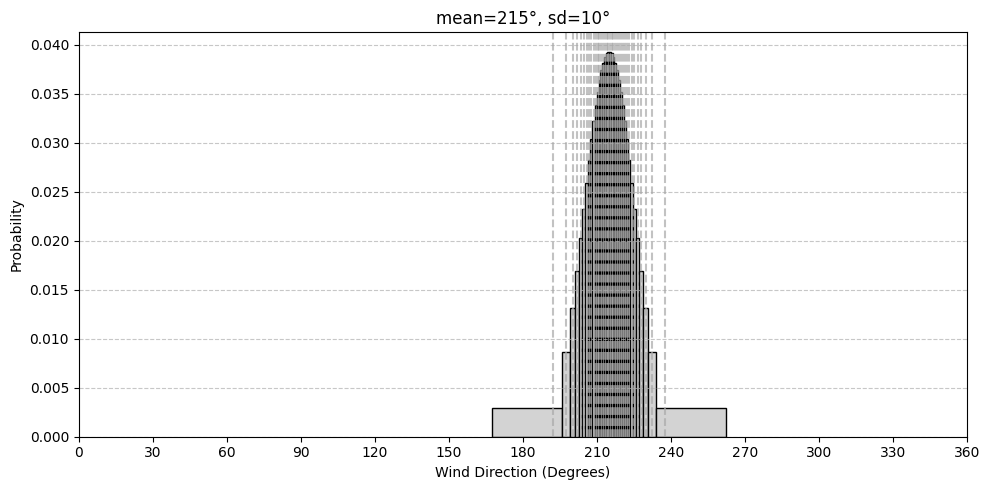
\includegraphics[width=0.8\textwidth]{../figures/optimization/stoch2/dist_discret.png} 
	\caption{Quantile based discretized Normal with mean 260° and standard deviation 10°, discretized for 35 quantiles}
	\label{fig:stoch2_dist}
\end{figure} 

With the parameter grid defined, the simulations can be performed, joint with the wind condition probabilities and expectations for the farm power calculated, yielding the dataset to be used in the training of the Neural Network. We thus proceed to the grid search optimization of the Neural Network configuration, as done in the previous chapters. For the distribution shown above, we find the 2-hidden layer and 20 neurons per hidden layer $\text{NN}(5\,{-}\,20^{\times2}\,{-}\,1)$ configuration to yield the best results for least numbers of neurons, as can be seen in Figure \ref{fig:stoch2_NNopti}. \textit{We thus proceed with the configuration $\text{NN}(5\,{-}\,20^{\times2}\,{-}\,1)$}.


\begin{figure}[h] 
	\centering
	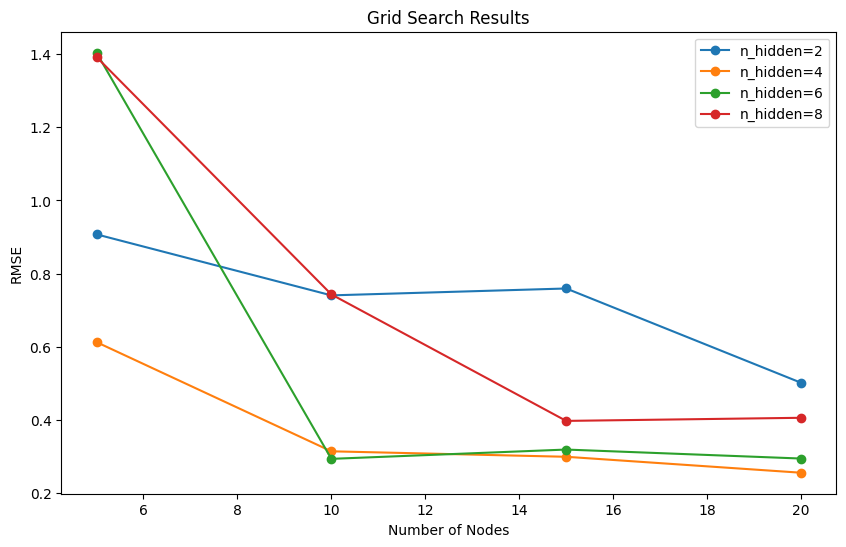
\includegraphics[width=0.8\textwidth]{../figures/optimization/stoch2/stoch2_NNopti.png} 
	\caption{Grid Search Results for models trained on Farm Power Expectation data, with parameter grid as defined in Table 	\ref{tab:val_prob2_data} and Figure  \ref{fig:stoch2_dist} }
	\label{fig:stoch2_NNopti}
\end{figure} 


The model of configuration $\text{NN}(5\,{-}\,20^{\times2}\,{-}\,1)$ is thus trained and a brief visual inspection performed to investigate how well the model fits the data. As shown in Figure \ref{fig:stoch2_heatmap_inspect_NN}, does the model encorporate the shape of the Expected Power Distribution across x/y fairly well, with the only major deviations near the orgin, e.g. the position of Turbine 1 and directly after Turbine 1 in the principal wind direction. 

\begin{figure}[h] 
	\centering
	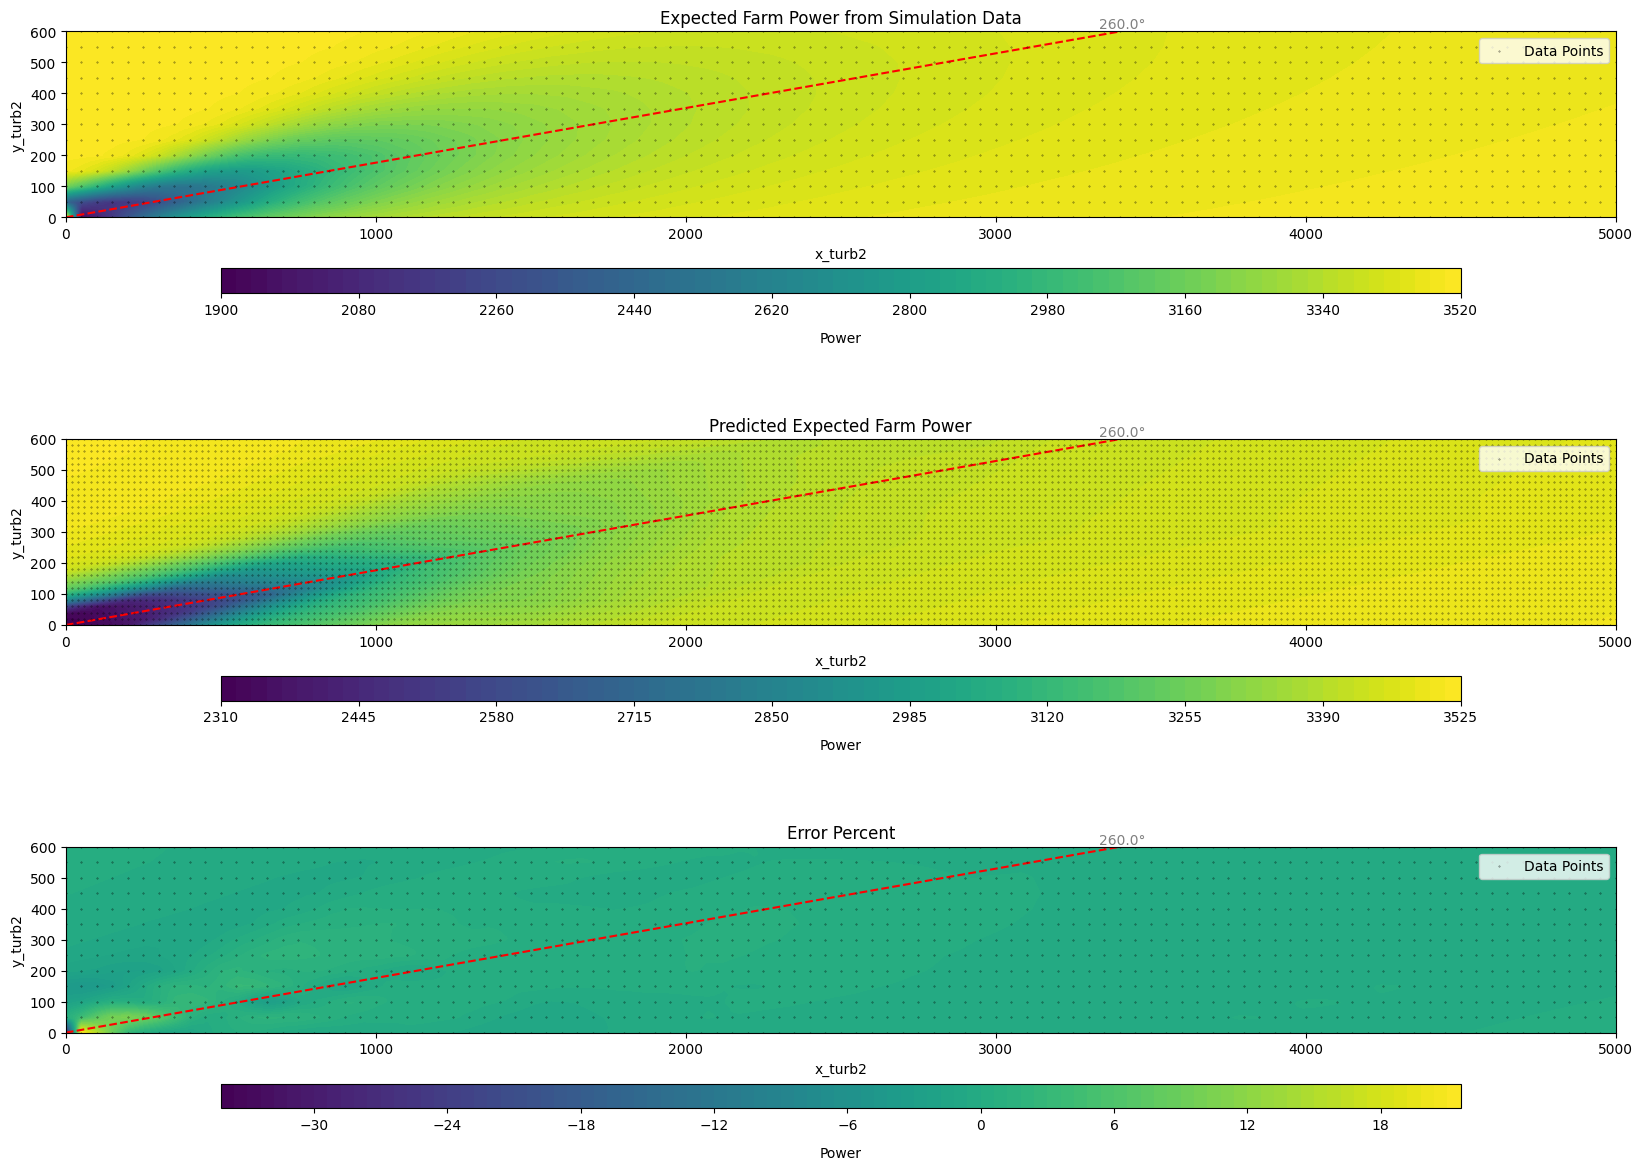
\includegraphics[width=1\textwidth]{../figures/optimization/stoch2/stoch2_heatmap_inspect_NN.png} 
	\caption{Visual comparison of training data vs predictions for Neural Network for Expectation of Farm Power, with linear interpolation in between data points to generate heatmap}
	\label{fig:stoch2_heatmap_inspect_NN}
\end{figure} 

The model thus appears to fit the physical behavior suficiently well to be able to proceed to the optimization step. 



\paragraph{Optimization}

The set up model is thus again embedded into a now seemingly deterministic optimization problem, as the uncertainty has already been taken into account when setting up the Neural Network itself through the expectations. The Neural Network is thus embedded directly into the problem, with the constraints as initially defined. The result shown in Figure \ref{fig:stoch2_opti} yield the expected result, with turbine 2 being placed as far upstream and as far away perpendicularly to the principal wind direction as possible from Wind Turbine 2. 

\begin{figure}[h] 
	\centering
	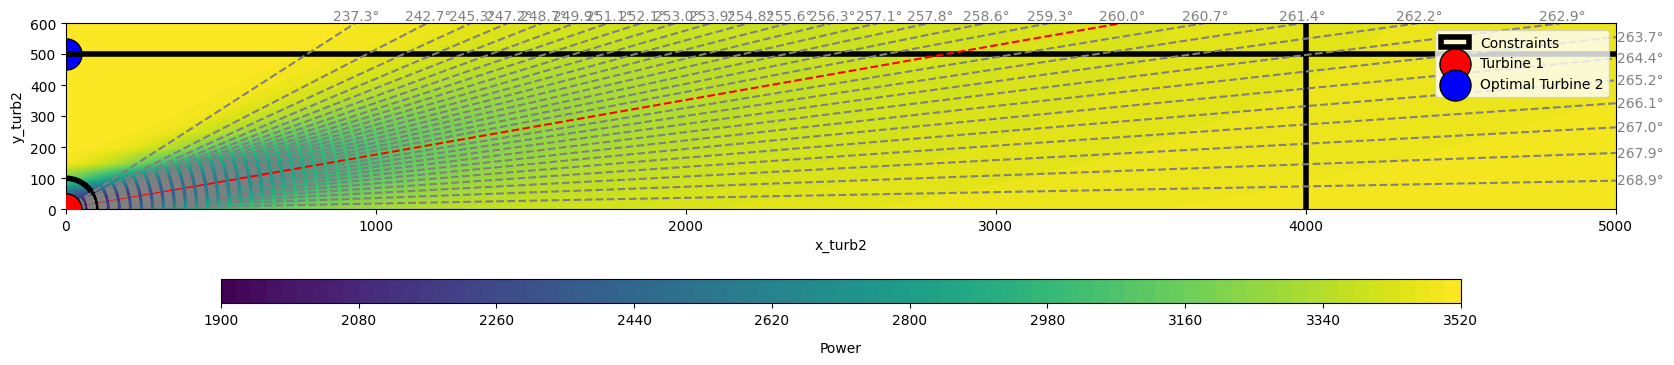
\includegraphics[width=1\textwidth]{../figures/optimization/stoch2/stoch2_opti.png} 
	\caption{Optimization Result for maximization of Expected Farm Power, with wind direction Normally distributed with mean 260° and standard deviation 10°, discretized into 35 scenarios using quantile based discretization and Neural Network configuration $\text{NN}(5\,{-}\,20^{\times2}\,{-}\,1)$ }
	\label{fig:stoch2_opti}
\end{figure} 

Notably, the solving of this variation optimization problem requires significantly less computational recourses as the previous stochastic formulation, with a significantly larger quantity of scenarios considered for calculating the Expectation. In the entire optimization pipeline, the main limitation is in this formulation constitued by running the simulations required for the individual discretization of different wind direction/wind condition distributions. Due to the efficency of the FLORIS simulations, this does not seem to be a limitation for the two turbine configuration at this moment however. Therefore, this method appears to be better fit to scale up the complexity of the wind condition distribution, allowing for expanding to a multivariate distribution of the potentially dependent variables wind direction and wind speed for example. 



\section{Conclusion}\label{chapter:conclusion}

The Thesis contains the training of a Neural Network to predict the total farm power/expected farm power generated by a wind farm consisting of two turbines, with the inputs to the model as the relative position of the second wind turbine to the first as well as the wind condition parameters like wind direction. The resulting Neural Networks where embedded into a mixed integer linear programming problem using an approach for decomposing a Neural Network into lmixed-integer inear constraints. Multiple optimization problems where solved using this aproach, beginning with a deterministic problem by only considering a dominant wind direction to find maxima for the total farm power. The formulation was then expanded to stochastic optimizations with a scenario based approach, to maximize the expected power generation, subject to a discreitzed distribution of the wind direction. Here two variants where developed, one via a large general neural network with the wind condition parameters as additional variables and one via a reduced Neural Network, trained on the already evaluated expected farm power for each x/y position of the second turbine. 

While the deterministic approach could be quickly discarded as insufficient, both of the stochastic formulations yielded benefits and drawbacks. The first formulation, using a larger Neural Network indipendent of the wind condition distribution yielded a versatile variant, with a Neural Network that could be applied to any location and any wind condition distribution, while only being able to consider a low number of scenarios due to computational constraints. The second stochastic formulation evaded the computational limitations by training its model directly on the farm power expectations, making both the Neural Network and the optimization model significantly more efficient, but loosing generality due to the Neural Networks conditioning on the wind condistion distribution.

Overall, the second stochastic formulation appears to be the only variant that sufficiently considers the randomness of the wind conditions like wind speed, while showing a path to scaling up computationally. In any case, results from both stochastic formulations where able to show how insufficient it would be to only consider a deterministic formulation.

With especially the second stochastic formulation having shown to deliver good results in this thesis, the next steps would revolve around investigating how to generalize the formulation to a larger number of wind turbines. Here, a fundamental reformulation might be required as the current formulation using relative positions would quickly grow the parameter space exponentially. 

None the less it might be worthwile to pursue as the underlying Constraint Learning Methodology has been shown to be able to cope with the complexity of wind turbine wakes in this Thesis.

\begin{thebibliography}{00}

%% For authoryear reference style
%% \bibitem[Author(year)]{label}
%% Text of bibliographic item

\bibitem[European Commission(2023)]{EU_RE_Targets_2023}
European Commission,
\textit{Renewable energy targets},
\url{https://energy.ec.europa.eu/topics/renewable-energy/renewable-energy-directive-targets-and-rules/renewable-energy-targets_en},
2023.
Accessed: 2025-04-03.

\bibitem[Analysis and Research Team(2024)]{ConsiliumEU_Harnessing_Wind_Power_2024}
Analysis and Research Team, General Secretariat of the Council of the European Union,
\textit{Harnessing Wind Power: Navigating the EU Energy Transition and Its Challenges},
\url{https://www.consilium.europa.eu/media/1kyk0wjm/2024_685_art_windpower_web.pdf},
September 2024.
Accessed: 2025-04-03.

\bibitem[European Environment Agency(2009)]{EEA_Wind_Energy_Potential_2009}
European Environment Agency,
\textit{Europe's Onshore and Offshore Wind Energy Potential},
Technical report 6/2009,
\url{https://www.eea.europa.eu/en/analysis/publications/europes-onshore-and-offshore-wind-energy-potential},
2009.
Accessed: 2025-04-03.

\bibitem[Nielsen(2015)]{nielsen2015neuralChap1}
Michael Nielsen,
\textit{Neural Networks and Deep Learning - Chapter 1},
\url{http://neuralnetworksanddeeplearning.com/chap1.html},
2015.
Accessed: 2025-04-10.

\bibitem[Nielsen(2015)]{nielsen2015neuralChap2}
Michael Nielsen,
\textit{Neural Networks and Deep Learning - Chapter 2: How the backpropagation algorithm works},
\url{http://neuralnetworksanddeeplearning.com/chap2.html},
2015.
Accessed: 2025-05-01.

\bibitem[James et al.(2023)]{James2023}
Gareth James and Daniela Witten and Trevor Hastie and Robert Tibshirani and Jonathan Taylor,
\textit{An Introduction to Statistical Learning: with Applications in Python},
Springer,
Springer Texts in Statistics,
2023,
ISBN 978-3-031-38747-0.

\bibitem[Alcántara and Ruiz(2023)]{ALCANTARA2023120895}
Antonio Alcántara and Carlos Ruiz,
\textit{A neural network-based distributional constraint learning methodology for mixed-integer stochastic optimization},
Expert Systems with Applications,
Volume 232,
2023.

\bibitem[Fajemisin et al.(2024)]{FAJEMISIN20241}
Adejuyigbe O. Fajemisin and Donato Maragno and Dick den Hertog,
\textit{Optimization with constraint learning: A framework and survey},
European Journal of Operational Research,
Volume 314,
Number 1,
Pages 1-14,
2024.

\bibitem[Vanderbei(2020)]{vanderbei2020chapter3}
Robert J. Vanderbei,
\textit{Linear Programming},
Chapter 3,
Springer,
5th edition,
2020.

\bibitem[Windpower Monthly(2019)]{windpowermonthly_offshore_clusters}
Windpower Monthly,
\textit{Offshore Wind Clusters to Lower Energy Production - Study},
\url{https://www.windpowermonthly.com/article/1719266/offshore-wind-clusters-to-lower-energy-production-–-study},
2019.
Accessed: 2025-04-29.

\bibitem[Kiranoudis and Maroulis(1997)]{KIRANOUDIS1997439}
C.T. Kiranoudis and Z.B. Maroulis,
\textit{Effective short-cut modelling of wind park efficiency},
Renewable Energy,
Volume 11,
Number 4,
Pages 439-457,
1997.

\bibitem[Magnusson and Smedman(1999)]{MAGNUSSON1999169}
M. Magnusson and A.-S. Smedman,
\textit{Air flow behind wind turbines},
Journal of Wind Engineering and Industrial Aerodynamics,
Volume 80,
Number 1,
Pages 169-189,
1999.

\bibitem[Bortolotti et al.(2019)]{Bortolotti2019}
Pietro Bortolotti and Helena Canet Tarrés and Katherine Dykes and Karl Merz and Latha Sethuraman and David Verelst and Frederik Zahle,
\textit{IEA Wind Task 37 on Systems Engineering in Wind Energy - WP2.1 Reference Wind Turbines},
National Renewable Energy Laboratory,
2019.

\bibitem[Madsen et al.(2022)]{Madsen2022}
Mads Madsen and Frederik Zahle and Sergio Gonzalez Horcas and Thanasis Barlas and Niels Sørensen,
\textit{CFD-based curved tip shape design for wind turbine blades},
Wind Energy Science,
Volume 7,
Pages 1471-1501,
2022.

\bibitem[Kainz et al.(2024)]{Kainz2024IEA}
Samuel Kainz and Julian Quick and Mauricio Souza de Alencar and Sebastian Sanchez Perez Moreno and Katherine Dykes and Christopher Bay and Michiel Zaaijer and Pietro Bortolotti,
\textit{IEA Wind TCP Task 55: The IEA Wind 740-10-MW Reference Offshore Wind Plants},
National Renewable Energy Laboratory,
NREL/TP-5000-87923,
2024.

\bibitem[Birge and Louveaux(1997)]{BirgeLouveauxStochasticProgramming}
John R. Birge and François Louveaux,
\textit{Introduction to Stochastic Programming},
Springer Series in Operations Research and Financial Engineering,
Springer,
1997.

\bibitem[Akpabio and Savari(2022)]{Akpabio}
Inimfon Akpabio and Serap Savari,
\textit{On the Construction of Distribution-Free Prediction Intervals for an Image Regression Problem in Semiconductor Manufacturing},
arXiv:2203.03150,
2022.

\bibitem[Marcjasz et al.(2023)]{Marcjasz_2023}
Grzegorz Marcjasz and Michał Narajewski and Rafał Weron and Florian Ziel,
\textit{Distributional neural networks for electricity price forecasting},
Energy Economics,
Volume 125,
2023.

\bibitem[Steinwart and Christmann(2011)]{Steinwart_2011}
Ingo Steinwart and Andreas Christmann,
\textit{Estimating conditional quantiles with the help of the pinball loss},
Bernoulli,
Volume 17,
Number 1,
2011.

\bibitem[Hou et al.(2019)]{hou_review_2019}
Peng Hou and Jiangsheng Zhu and Kuichao Ma and Guangya Yang and Weihao Hu and Zhe Chen,
\textit{A review of offshore wind farm layout optimization and electrical system design methods},
Journal of Modern Power Systems and Clean Energy,
Volume 7,
Number 5,
Pages 975-986,
2019.

\bibitem[Kim et al.(2024)]{KIM2024123383}
Taewan Kim and Jeonghwan Song and Donghyun You,
\textit{Optimization of a wind farm layout to mitigate the wind power intermittency},
Applied Energy,
Volume 367,
2024.

\bibitem[Azlan et al.(2021)]{AZLAN2021110047}
F. Azlan and J.C. Kurnia and B.T. Tan and M.-Z. Ismadi,
\textit{Review on optimisation methods of wind farm array under three classical wind condition problems},
Renewable and Sustainable Energy Reviews,
Volume 135,
2021.

\bibitem[Wang et al.(2024)]{WANG2024118508}
Li Wang and Mi Dong and Jian Yang and Lei Wang and Sifan Chen and Neven Duić and Young Hoon Joo and Dongran Song,
\textit{Wind turbine wakes modeling and applications: Past, present, and future},
Ocean Engineering,
Volume 309,
2024.

\bibitem[Yang et al.(2023)]{YANG2023119240}
Kun Yang and Xiaowei Deng and Zilong Ti and Shanghui Yang and Senbin Huang and Yuhang Wang,
\textit{A data-driven layout optimization framework of large-scale wind farms based on machine learning},
Renewable Energy,
Volume 218,
2023.

\bibitem[Bempedelis et al.(2024)]{wes-9-869-2024}
N. Bempedelis and F. Gori and A. Wynn and S. Laizet and L. Magri,
\textit{Data-driven optimisation of wind farm layout and wake steering with large-eddy simulations},
Wind Energy Science,
Volume 9,
Number 4,
Pages 869-882,
2024.

\bibitem[Ti et al.(2020)]{TI2020114025}
Zilong Ti and Xiao Wei Deng and Hongxing Yang,
\textit{Wake modeling of wind turbines using machine learning},
Applied Energy,
Volume 257,
2020.

\bibitem[Ti et al.(2021)]{TI2021618}
Zilong Ti and Xiao Wei Deng and Mingming Zhang,
\textit{Artificial Neural Networks based wake model for power prediction of wind farm},
Renewable Energy,
Volume 172,
Pages 618-631,
2021.

\bibitem[Alcántara et al.(2025)]{ALCANTARA2025127876}
Antonio Alcántara and Carlos Ruiz and Calvin Tsay,
\textit{A quantile neural network framework for two-stage stochastic optimization},
Expert Systems with Applications,
2025.

\bibitem[De Raedt et al.(2018)]{de2018learning}
Luc De Raedt and Andrea Passerini and Stefano Teso,
\textit{Learning constraints from examples},
Proceedings of the AAAI conference on artificial intelligence,
Volume 32,
2018.

\bibitem[Bonfietti et al.(2015)]{preprintBonfiettiEmbeddDecisionTrees}
Alessio Bonfietti and Michele Lombardi and Michela Milano,
\textit{Embedding Decision Trees and Random Forests in Constraint Programming},
2015.

\bibitem[de-Alba et al.(2024)]{dealba2024reformulationembeddingneuralnetwork}
Héctor G. -de-Alba and Andres Tellez and Cipriano Santos and Emmanuel Gómez,
\textit{A reformulation to Embedding a Neural Network in a linear program without integer variables},
arXiv:2402.02086,
2024.

\bibitem[Sinner and Fleming(2024)]{Sinner_2024}
Michael Sinner and Paul Fleming,
\textit{Robust wind farm layout optimization},
Journal of Physics: Conference Series,
Volume 2767,
Number 3,
2024.

\bibitem[Glorot et al.(2010)]{preprintReLuGlorot}
Xavier Glorot and Antoine Bordes and Y. Bengio,
\textit{Deep Sparse Rectifier Neural Networks},
Journal of Machine Learning Research,
Volume 15,
2010.

\bibitem[NREL(2025)]{nrel_floris}
National Renewable Energy Laboratory (NREL),
\textit{FLORIS: FLOw Redirection and Induction in Steady State},
GitHub repository,
Version 4.4.2,
\url{https://github.com/NREL/floris},
2025.

\bibitem[NREL(2025)]{nrel_floris_web}
National Renewable Energy Laboratory (NREL),
\textit{FLORIS: FLOw Redirection and Induction in Steady State},
\url{https://www.nrel.gov/wind/floris},
March 2025.

\bibitem[Pedersen et al.(2025)]{dtu_pywake_2025}
Mads M. Pedersen and Paul van der Laan and Mikkel Friis-Møller and Alexander Meyer Forsting and Riccardo Riva and Leonardo Andrés Alcayaga Román and Javier Criado Risco and Julian Quick and Jens Peter Schøler Christiansen and Bjarke Tobias Olsen and Rafael Valotta Rodrigues and Pierre-Elouan Réthoré,
\textit{PyWake: an open-source Python wind farm simulation tool},
\url{https://topfarm.pages.windenergy.dtu.dk/PyWake/},
2025.

\bibitem[Schmetz(2025)]{schmetz2025_gendata_git}
Simon Schmetz,
\textit{generate\_data\_floris.ipynb - Wind Farm Power Modelling},
\url{https://github.com/schmeti/uc3m_TFM_wind_farm_optimization_codebase/blob/main/Windfarm_power_modelling/generate_data_floris.ipynb},
2025.
Accessed: 2025-06-06.

\bibitem[Alcantara and Ruiz(2022)]{alcantara_ruiz_distcl_2022_git}
Antonio Alcantara and Carlos Ruiz,
\textit{DistCL: A Neural Network-Based Distributional Constraint Learning tool for Mixed-Integer Stochastic Optimization},
\url{https://github.com/antonioalcantaramata/DistCL},
2022.
Accessed: 2025-06-06.

\bibitem[Schmetz(2025)]{schmetz2025twoturbine_determ}
Simon Schmetz,
\textit{Two-Turbine Wind Farm Optimization using Constrained Learning (Deterministic)},
\url{https://github.com/schmeti/uc3m_TFM_wind_farm_optimization_codebase/blob/main/Windfarm_power_modelling/0_two_turbine_problem_constrLearn_determin.ipynb},
2025.
Accessed: 2025-06-06.

\bibitem[Schmetz(2025)]{schmetz2025twoturbine_stoch1}
Simon Schmetz,
\textit{Two-Turbine Problem with Constraint Learning and Probability-Weighted Objective},
\url{https://github.com/schmeti/uc3m_TFM_wind_farm_optimization_codebase/blob/main/Windfarm_power_modelling/0_two_turbine_problem_constrLearn_probweighted.ipynb},
2025.
Accessed: 2025-06-06.

\bibitem[Schmetz(2025)]{schmetz2025twoturbine_stoch2}
Simon Schmetz,
\textit{Two-Turbine Problem with Constraint Learning and Probability-Weighted Objective (Expectation Neural Network)},
\url{https://github.com/schmeti/uc3m_TFM_wind_farm_optimization_codebase/blob/main/Windfarm_power_modelling/0_two_turbine_problem_constrLearn_probweightedt_expNN.ipynb},
2025.
Accessed: 2025-06-06.


\end{thebibliography}
\end{document}

\endinput
%%
%% End of file `elsarticle-template-num-names.tex'.
